%% This is the ctufit-thesis example file. It is used to produce theses
%% for submission to Czech Technical University, Faculty of Information Technology.
%%
%% Get the newest version from
%% https://gitlab.fit.cvut.cz/theses-templates/FITthesis-LaTeX
%%
%%
%% Copyright 2021, Eliska Sestakova and Ondrej Guth
%%
%% This work may be distributed and/or modified under the
%% conditions of the LaTeX Project Public Licenese, either version 1.3
%% of this license or (at your option) any later version.
%% The latest version of this license is in
%%  https://www.latex-project.org/lppl.txt
%% and version 1.3 or later is part of all distributions of LaTeX
%% version 2005/12/01 or later.
%%
%% This work has the LPPL maintenance status `maintained'.
%%
%% The current maintainer of this work is Ondrej Guth.
%% Contact ondrej.guth@fit.cvut.cz for bug reports.
%% Alternatively, submit bug reports into the tracker at
%% https://gitlab.fit.cvut.cz/theses-templates/FITthesis-LaTeX/issues
%%
%%

%%%%%%%%%%%%%%%%%%%%%%%%%%%%%%%%%%%%%%%%%
% CLASS OPTIONS
% language: czech/english/slovak
% thesis type: bachelor/master/dissertation
%%%%%%%%%%%%%%%%%%%%%%%%%%%%%%%%%%%%%%%%%
\documentclass[english,bachelor,unicode]{ctufit-thesis}

%%%%%%%%%%%%%%%%%%%%%%%%%%%%%%%%%%
% FILL IN THIS INFORMATION
%%%%%%%%%%%%%%%%%%%%%%%%%%%%%%%%%%
\ctufittitle{Spatial sound for immersive video} % replace with the title of your thesis
\ctufitauthorfull{Ivan Desiatov} % replace with your full name (first name(s) and then family name(s) / surname(s)) including academic degrees
\ctufitauthorsurnames{Desiatov} % replace with your surname(s) / family name(s)
\ctufitauthorgivennames{Ivan} % replace with your first name(s) / given name(s)
\ctufitsupervisor{Ing.\,Jan Buriánek} % replace with name of your supervisor/advisor (include academic degrees)
\ctufitdepartment{Department of Software Engineering} % replace with the department of your defence
\ctufityear{2022} % replace with the year of your defence
\ctufitdeclarationplace{Prague} % replace with the place where you sign the declaration
\ctufitdeclarationdate{\today} % replace with the date of signature of the declaration
\ctufitabstractCZE{
    Práce představuje nejvýznamnější moderní technologie ve sféře prostorového audia
    a uvádí výhody, díky kterým ambisonie začíná být standardním formátem zvuku pro 360\degree{}~video.
    Práce uvádí čtenáře do teoretických základů ambisonie a popisuje několik důležitých dekódovacích technik.
    Následně je představeno softwarové řešení umožňující automatické prostorové panorámování zvuku v DAW
    na základě 3D pozicí objektů (vůči aktivní kameře) ve scéně v Blenderu.
    Implementace obsahuje dva pluginy - plugin pro Blender, umožňující
    přístup k současnému stavu 3D scény, a VST plugin, který využívá tyto informace o 3D scéně pro ambisonické panorámování zvuku.
    Panoramovácí směrové vektory jsou aktualizovaný v reálném čase pomoci meziprocesové komunikace.
    Umělcům a inženýrům pracujícím na projektu to pak dovoluje mít před sebou náhled animace a současně provádět změny v audiu,
    a obráceně - slyšet, jak změny v poloze objektů ovlivňují zvuk.
    Představené řešení je nejužitečnější pro produkci prostorového zvuku pro 360\degree{} 3D animace,
    kde může výrazně snížit počet kanálů vyžadujících ruční panoramování.
    Najde ale využití i v neanimovaných projektech, kde může sloužit k vizualizaci pohybu zdrojů zvuku,
    a umožní využití dostupných v Blenderu pokročilých nástrojů pro 3D animaci.
}
\ctufitabstractENG{
    This thesis provides an overview of modern immersive audio technologies and outlines why ambisonics 
    is becoming the industry-standard spatial audio format for 360\degree{} video. 
    An introduction to ambisonics theory is provided, and several important decoding techniques are described. 
    A software solution is then presented, which implements automatic spatial panning of sounds in a DAW based on the 3D positions of objects (relative to the active camera) in the Blender scene.
    The implementation consists of two plugins - a Blender plugin to access the 3D scene data, and a VST ambisonic panner plugin that utilises said scene data to calculate the panning direction.
    Panning direction vectors are updated in real time using interprocess communication, allowing artists to preview the animation while simultaneously making adjustments to the audio, and vice versa.
    The presented solution is especially useful in producing spatial audio for 360\degree{} 3D animations, where it can help reduce the number of audio sources that have to be panned manually.
    It can however find a place in non-animated projects as well, where it can be used to visualise the movement of sound sources, and would allow to use Blender's advanced 3D animation toolset
    for animating sound source positions.
}
\ctufitkeywordsCZE{ambisonie, prostorový zvuk, blender, 360 stupňové video, virtualní realita, digital audio workstation, VST, plugin, JUCE, meziprocesová komunikace}
\ctufitkeywordsENG{ambisonics, spatial audio, blender, 360 degree video, virtual reality, digital audio workstation, VST, plugin, JUCE, inter-process communication}
%%%%%%%%%%%%%%%%%%%%%%%%%%%%%%%%%%
% END FILL IN
%%%%%%%%%%%%%%%%%%%%%%%%%%%%%%%%%%

%%%%%%%%%%%%%%%%%%%%%%%%%%%%%%%%%%
% CUSTOMIZATION of this template
% Skip this part or alter it if you know what you are doing.
%%%%%%%%%%%%%%%%%%%%%%%%%%%%%%%%%%

\RequirePackage{iftex}[2020/03/06]
\iftutex % XeLaTeX and LuaLaTeX
    \RequirePackage{ellipsis}[2020/05/22] %ellipsis workaround for XeLaTeX
\else
    \RequirePackage[utf8]{inputenc}[2018/08/11] %this file encoding
    \RequirePackage{lmodern}[2009/10/30] % vector flavor of Computer Modern font
\fi

% hyperlinks
\RequirePackage[pdfpagelayout=TwoPageRight,colorlinks=false,allcolors=decoration,pdfborder={0 0 0.1}]{hyperref}[2020-05-15]

% uncomment the following to hide all hyperlinks
% \RequirePackage[pdfpagelayout=TwoPageRight,hidelinks]{hyperref}[2020-05-15]

\RequirePackage{pdfpages}[2020/01/28]

\setcounter{secnumdepth}{4} % numbering sections; 4: subsubsection

%%%%%%%%%%%%%%%%%%%%%%%%%%%%%%%%%%
% CUSTOMIZATION of this template END
%%%%%%%%%%%%%%%%%%%%%%%%%%%%%%%%%%


%%%%%%%%%%%%%%%%%%%%%%
% DEMO CONTENTS SETTINGS
% You may choose to modify this part.
%%%%%%%%%%%%%%%%%%%%%%
\usepackage{gensymb}
\usepackage{dirtree}
\usepackage{lipsum,tikz}
\usepackage{csquotes}
\usepackage{float}
\usepackage[style=iso-numeric]{biblatex}
% \usepackage{listings} % typesetting of source code
\usepackage{minted} % typesetting of source code
\usepackage{graphicx}
\usepackage{bm}
\usepackage{wrapfig}
\usepackage{enumitem}
\usepackage{array}

\graphicspath{images}

%theorems, definitions, etc.
\theoremstyle{plain}
\newtheorem{theorem}{Věta}
\newtheorem{lemma}[theorem]{Tvrzení}
\newtheorem{corollary}[theorem]{Důsledek}
\newtheorem{proposition}[theorem]{Návrh}
\newtheorem{definition}[theorem]{Definice}
\theoremstyle{definition}
\newtheorem{example}[theorem]{Příklad}
\theoremstyle{remark}
\newtheorem{note}[theorem]{Poznámka}
\newtheorem*{note*}{Poznámka}
\newtheorem{remark}[theorem]{Pozorování}
\newtheorem*{remark*}{Pozorování}
\numberwithin{theorem}{chapter}

\newlist{funcreqs}{enumerate}{2}
\setlist[funcreqs, 1]{label = \textbf{FR\arabic*:}, leftmargin=*}
\setlist[funcreqs, 2]{label = FR\arabic{funcreqi}.\arabic*, leftmargin=*}
\newlist{nonfuncreqs}{enumerate}{2}
\setlist[nonfuncreqs, 1]{label = \textbf{NFR\arabic*:}, leftmargin=*}
\setlist[nonfuncreqs, 2]{label = NFR\arabic{funcreqi}.\arabic*, leftmargin=*}

%theorems, definitions, etc. END
%%%%%%%%%%%%%%%%%%%%%%
% DEMO CONTENTS SETTINGS END
%%%%%%%%%%%%%%%%%%%%%%

% \bibliography{text/bib-database}
\addbibresource{bib-database.bib}

\begin{document} 

\newmint{cpp}{}
\newmintinline{cpp}{}
\newmint{python}{}
\newmintinline{python}{}

\frontmatter\frontmatterinit % do not remove these two commands

\includepdf{zadani_bp-include.pdf} % replace that file with your thesis assignment provided by study office

\thispagestyle{empty}\cleardoublepage\maketitle % do not remove these three commands

\imprintpage % do not remove this command

\tableofcontents % do not remove this command
%%%%%%%%%%%%%%%%%%%%%%
% list of other contents: figures, tables, code listings, algorithms, etc.
% add/remove commands accordingly
%%%%%%%%%%%%%%%%%%%%%%
\listoffigures % list of figures
\begingroup
\let\clearpage\relax
\listoftables % list of tables
% \lstlistoflistings % list of source code listings generated by the listings package
\listoflistings % list of source code listings generated by the minted package
\endgroup
%%%%%%%%%%%%%%%%%%%%%%
% list of other contents END
%%%%%%%%%%%%%%%%%%%%%%

%%%%%%%%%%%%%%%%%%%
% ACKNOWLEDGMENT
% FILL IN / MODIFY
% This is a place to thank people for helping you. It is common to thank your supervisor.
%%%%%%%%%%%%%%%%%%%
\begin{acknowledgmentpage}
	I would like to thank my thesis mentor, Jan Buriánek, for providing advice and valuable industry insight,
    as well as the people who have supported me throughout the process of putting this together; you know who you are.
\end{acknowledgmentpage} 
%%%%%%%%%%%%%%%%%%%
% ACKNOWLEDGMENT END
%%%%%%%%%%%%%%%%%%%


%%%%%%%%%%%%%%%%%%%
% DECLARATION
% FILL IN / MODIFY
%%%%%%%%%%%%%%%%%%%
% INSTRUCTIONS
% ENG: choose one of approved texts of the declaration. DO NOT CREATE YOUR OWN. Find the approved texts at https://courses.fit.cvut.cz/SFE/download/index.html#_documents (document Declaration for FT in English)
% CZE/SLO: Vyberte jedno z fakultou schvalenych prohlaseni. NEVKLADEJTE VLASTNI TEXT. Schvalena prohlaseni najdete zde: https://courses.fit.cvut.cz/SZZ/dokumenty/index.html#_dokumenty (prohlášení do ZP)
\begin{declarationpage}
I  hereby  declare  that  the  presented  thesis  is  my  own \
work  and  that  I  have  cited  all sources  of  information  in  accordance  with  the  Guideline  for  adhering  to  ethical principles when elaborating an academic final thesis. I acknowledge that my thesis is subject to the rights and obligations stipulated by the Act No. 121/2000 Coll., the Copyright Act, as amended. In accordance with Article 46(6) of  the  Act,  I  hereby  grant  a  nonexclusive  authorization  (license)  to  utilize  this  thesis, including any and all computer programs incorporated therein or attached thereto and all corresponding documentation (hereinafter collectively referred to as the “Work”), to any and all persons that wish to utilize the Work. Such persons are entitled to use the Work for non-profit purposes only, in any way that does not detract from its value. This authorization is not limited in terms of time, location and quantity.
\end{declarationpage}
%%%%%%%%%%%%%%%%%%%
% DECLARATION END
%%%%%%%%%%%%%%%%%%%

\printabstractpage % do not remove this command

%%%%%%%%%%%%%%%%%%%
% ABBREVIATIONS
% FILL IN / MODIFY
% OR REMOVE ENTIRELY
% List the abbreviations in lexicography order.
%%%%%%%%%%%%%%%%%%%
\chapter{List of abbreviations}
% A B C D E F G H I J K L M N O P Q R S T U V W X Y Z
\begin{tabular}{rl}
API & Application Programming Interface\\
AR & Augmented Reality\\
CBA & Channel-based Audio\\
DAW & Digital Audio Workstation\\
FIFO & First In, First Out\\
FFT & Fast Fourier Transform\\
FPS & First-Person Shooter\\
FPS & Frames per Second\\
GUI & Graphical User Interface\\
HCI & Human-Computer Interface\\
HRIR & Head-Related Impulse Response\\
HRTF & Head-Related Transfer Function\\
MR & Mixed Reality\\
M/S Stereo & Mid/Side Stereo\\
OBA & Object-based Audio\\
SBA & Scene-based Audio\\
SDK & Software Development Kit\\
VR & Virtual Reality\\
VST & Virtual Studio Technology\\
UI & User Interface\\
UX & User Experience\\
% XR & Extended Reality\\
\end{tabular}
%%%%%%%%%%%%%%%%%%%
% ABBREVIATIONS END
%%%%%%%%%%%%%%%%%%%

\chapter{Introduction}

\section*{Virtual reality and immersive video}
Virtual reality, or VR, has become increasingly popular in recent years. 
VR gaming specifically has been steadily rising to mainstream attention. 
But other forms of immersive content, such as 360\degree{} video 
are also gaining adoption - YouTube, for example, already provides support for 360\degree{} video
(and audio) on their platform.

The goal of VR experiences is to fully immerse the user in a virtual environment, striving to erase the gap between the virtual and the real world.
This is achieved using advanced human-computer interfaces. Most prominently - VR headsets, that allow the user to see into the virtual world, 
and various motion tracking systems, enabling the user to interact with it.
Like any new form of human-computer interaction, VR has found applications in many industries,
but the application most closely related to the goal of this thesis, and, incidentally, the one where most adoption has been seen so far, is entertainment.

While fully interactive experiences, such as games, are prevalent, the applications of VR are not limited to those.
Immersive, or 360\degree{}, video
\footnote{Throughout this thesis I will prefer using ``360\degree{} video" instead of ``immersive video",
because, this being such a new concept, there is some inconsistency in terminology between some sources.}
is a mostly noninteractive form of VR content that benefits from the advantages of VR, 
but is closer to traditional film and television than other forms of immersive experiences such as games.

Creation of interactive VR experiences shares more similarity with game development than traditional video production.
360\degree{} video, on the other hand,
is largely linear, allowing to use creative software initially developed without VR content in mind.
Compared to specialized immersive content creation programs, such software
is often more powerful, costs less, and benefits from higher availability of learning resources regarding it's usage.
These factors would make it a great choice for creators, if not for the lacklustre VR content support.
Thankfully, many of these tools are extensible via plugins, allowing developers to fill in the gaps.

\section*{The role of sound in immersive experiences}
Sound is a key ingredient in achieving immersion in a virtual environment.
Although it's importance is easily outshined by the importance of sight, hearing is an essential part of human perception
and getting audio wrong in a VR context can easily ruin the whole experience.
While simulating the perception of touch - another vital sense - is a very difficult task, doing the same for hearing is fortunately already within our reach 
(although, as with real-time graphics, physically accurate techniques are still too computationally expensive).
To do so, as with video, the extension of audio into the third dimension is required.
Because of that, creating audio for an immersive experience is quite different to normal audio production.
In addition to the usual recording, sound design and mixing work, the spatial position of sounds must be defined and animated.

\section*{The goal of this thesis}
It might seem that to utilise the power of modern DAWs (digital audio workstations) for spatial audio production,
the DAW itself has to provide a user interface for spatial panning\footnote{Spatial panning refers to the act of defining the 3D position of a sound source.}
, be it natively or via plugins,
but a different approach may be taken.
Blender - a free and open source 3D software - already provides all the required tools and an established workflow for 3D animation.
The challenge lies in finding a way to utilise it's capabilities to control the spatial position of sounds while still using the DAW for sound design and mixing.
This can be achieved by extending both Blender and the DAW via plugins, allowing the user to use Blender's 3D animation workflow for spatial audio.
An existing 3D animation can also be used, providing significant time savings for animated 360\degree{} video productions.
This thesis aims to design and implement such a solution.

% \chapter*{The goals of this thesis}
% \begin{enumerate}
%     \item Review the current state of spatial audio technology.
%     \item Analyse available solutions for spatial audio production (with a focus on 360\degree{} video production).
%     \item Design a solution that will synchronize the spatial position of sounds in a DAW with the respective
%     positions of objects in a Blender scene in real time, and then allow to export the resulting audio.
%     \item Implement said solution, test it, and document it's functionality.
% \end{enumerate}


\mainmatter\mainmatterinit % do not remove these two commands

%%%%%%%%%%%%%%%%%%%
% THE THESIS
% MODIFY ANYTHING BELOW THIS LINE
%%%%%%%%%%%%%%%%%%%
\setcounter{page}{1}
\chapter{Spatial audio}

\begin{chapterabstract}
    This chapter serves as an introduction to spatial audio.
    Different approaches to representing spatial audio information are presented,
    and their suitability for 360\degree{} video applications is discussed.
    A more in-depth section on ambisonics follows, accompanied by a brief 
    foray into the mechanisms behind human spatial hearing.
\end{chapterabstract}

\section{Spatial audio representations}

There are three main approaches to representing spatial audio information -
channel-based audio, object-based audio and scene-based audio. \cite{ebu_sbo_hoa}\cite{mpeg_3d_article}\cite{sba_using_hoa}
Each with their own advantages and disadvantages for specific applications. Let me briefly introduce each paradigm. 

\subsection{Channel-based audio}
CBA content consists of a set of audio signals, each of them intended to feed a loudspeaker
at a specific position relative to the listener. \cite{mpeg_3d_article} 
It is extensively used for 3D sound in broadcasting and film \cite{ebu_sbo_hoa}\cite{mpeg_3d_article},
but it's core design is flawed in assuming a fixed speaker layout.
Reproducing channel based content on a speaker layout with a number of channels that is different to the one it was produced for
requires using sophisticated downmixing or upmixing algorithms which may result in loss of quality and spatial resolution. \cite{mpeg_3d_article}\cite{brinkman2015effect}
A study performed by researchers at the Delft University of Technology shows that Dolby Surround, which 
employs a downmixing technique \cite{dolby_digital} to playback surround audio on stereo headphones, 
showed significantly lower perceived ``overall presence" than even traditional stereo (not utilising HRTFs). \cite{hoekstra20133d}\cite{brinkman2015effect}
Furthermore, channel-based audio doesn't account for the possibility of speakers being positioned differently than the intended layout (an occurrence common in the real world),
which will inevitably alter the directionality of sounds and make the experience differ from the one intended by the content creator(s).

While CBA has been used extensively for delivering surround audio content in film and video games, it has a lot of constraints stemming 
from the assumption of a specific speaker count and layout made during the production stage. 
The most important constraint for VR applications is the difficulty in rotating the sound scene as a whole, 
which is required to keep the sound positions anchored in space while the listener's head may rotate.
While it can be done, the results are subpar at best, and result in ``\emph{a sound that goes in and out of focus
as the channels move into and out of particular speakers}" \cite[p.~45]{new_realities_in_audio}.

The other two spatial audio paradigms - OBA and SBA, don't share these flaws of CBA. \cite{ebu_sbo_hoa}\cite{system_for_oba}
Instead of relying on a specific speaker layout, they describe the audio scene independently of the playback hardware (the end user's speakers or headphones),
allowing playback on arbitrary loudspeaker setups while preserving spatial information and 
general audio quality better than CBA transformed using downmixing or upmixing techniques. \cite{system_for_oba}\cite{sba_using_hoa}

\subsection{Object-based audio}
OBA, which originated in game audio \cite{cambridge_imm_audio_review}, describes audio in a more general way. 
The content is represented as a virtual sound scene - a collection of sound sources called objects. \cite{ss_with_speakers_review}
An audio feed, as well as metadata, describing how the sound should be rendered, is assigned to each object. \cite{ss_with_speakers_review}\cite{cambridge_imm_audio_review}
This representation allows OBA content to be rendered on the end user's hardware, accounting for 
their specific (possibly non-standard \cite{oba_panner_patent}) speaker configuration,
as well as in the form of binaural audio, which will be described in more detail later. \cite{system_for_oba}\cite{cambridge_imm_audio_review}

OBA comes with it's own disadvantages - the main of which being the direct correlation
between the number of individual sound objects, the bandwidth required to transmit the OBA content, and decoding complexity. \cite{ebu_sbo_hoa}
There are however proposed solutions to lower the required bandwidth by employing object grouping techniques. \cite{breebaart2019spatial}

Object-based audio seems to be much better suited for VR applications than CBA.
It brings the ability to differentiate between individual audio objects 
and adjust their position relative to each other which is indispensable for VR games.
While the interactivity potential OBA brings is enticing, it is not as beneficial for noninteractive content, and
the increased bandwidth requirements are undesirable, especially for 360\degree{} video streaming scenarios.

\subsection{Scene-based audio}

While SBA still uses the concept of channels,
the channels play a very different role - instead of associating each channel with a specific speaker, as in CBA,
or with a specific sound object, as in OBA, the channels in SBA are combined to equally capture 
the sound coming from all directions. \cite{new_realities_in_audio}\cite{sba_using_hoa}\cite{cambridge_imm_audio_review}

Ambisonics is the underlying mathematical framework that makes SBA possible.
It is a surprisingly old approach 
initially described by Michael A. Gerzon in 1972 in his article ``Periphony: With-Height Sound Reproduction" \cite{gerzon1973periphony}.
Ambisonic content can easily be transformed to allow playback on any speaker arrangement, it is computationally viable to decode, encode,
and apply simple processing, such as rotating the sound scene,
in real time, and it's flexible in allowing to lower the required bandwidth at the cost of decreased spatial resolution. \cite{new_realities_in_audio}\cite{qualcomm_sba}
Ambisonics is in fact so powerful, and such a good fit for 360\degree{} video, that it gets a dedicated section.

\section{Ambisonics}

\subsection{M/S Stereo}

To understand how ambisonics make all of this possible, let's start with a simpler concept -
stereo audio, specifically it's Mid/Side representation.
When the term stereo is mentioned, most readers will probably associate it with X/Y encoding where the audio is encoded using a left and right channel.
This representation is natural for humans, because it closely resembles the way our hearing works, 
but mid/side (commonly shortened to M/S) encoding (\cite{ms_herre2004joint}) brings significant advantages compared to X/Y. 
It is very easily downmixed to mono, and gives the ability to widen or narrow the stereo image. \cite{new_realities_in_audio}

It's easiest to explain how M/S encoding works on a recording example.
To record M/S stereo one needs two microphones - one with a cardioid or omnidirectional pattern,
and a second microphone with a figure-eight pattern, positioned at a 90\degree{} angle relative to the first microphone. 
The first microphone captures sound from a wide area in front of the microphone or from all directions, this microphone will provide the mid channel signal.
A figure-eight pattern microphone captures sound predominantly in front and behind it,
so when rotated 90 degrees it will provide the necessary information for our side channel.
To get a stereo field, the side channel is duplicated and one of the copies is phase shifted 180\degree{}.
Let's refer to the phase shifted version as \emph{S-} and the original side channel as \emph{S+}.
The left channel can then be calculated as \emph{L = M + S+} and the right as \emph{R = M + S-}. 
In practice this means hard-panning
\footnote{In music production and audio mixing, hard-panning a channel means routing it exclusively to a single speaker.
    This approach was popular when stereo was first introduced, and can be heard, for example, on many The Beatles records.}
the \emph{S+} channel left, and hard-panning the \emph{S-} channel right.
Figure \ref{fig:ms_stereo} visualises the microphone setup and channel routing.
To get a mono version, one can just use the mid channel, and to widen or narrow the stereo image,
the relative volume of the side channel can be adjusted. \cite{ms_recording_basics}\cite{new_realities_in_audio}\cite{ambisonics_practical_theory}


\begin{figure}
    \begin{center}
        \includegraphics[height=20em]{images/spatial_audio/ms_stereo}       
        \caption{M/S stereo recording technique. Image sourced from \cite{recording_practices_wiki}. \label{fig:ms_stereo}}    
    \end{center}
\end{figure}

\subsection{From M/S stereo to B-format ambisonics}

The B-format is the minimal representation of ambisonics \cite{new_realities_in_audio}[p.~42]. It consists of four channels - 
\emph{W}, \emph{X}, \emph{Y} and \emph{Z}.
The role of the \emph{W} channel is analogous to the \emph{M} channel in M/S encoding - 
it captures sound coming from all directions equally. 
The other three channels - \emph{X}, \emph{Y} and \emph{Z} - are similar to the \emph{S} 
channel in M/S recording, but each one captures sound in a different plane,
the \emph{Y} channel - to the left and right of the listener, the \emph{X} channel - in front and behind,
and the \emph{Z} channel - above and below.
By distributing the source audio between the four channels, a sound can be positioned anywhere
on a sphere around the listener.
\cite{new_realities_in_audio}\cite{gerzon1973periphony}\cite{sba_using_hoa}

\subsection{Higher Order Ambisonics}
After the B-format was initially described, the mathematical framework
for ambisonics has been further extended, probably most notably by J{\'e}r{\^o}me 
Daniel when he described higher order ambisonics (HOA) in his Ph.D. thesis \cite{hoa_daniel}.
HOA extends the B-format by adding additional channels to increase the spatial resolution.
After the introduction of HOA, Gerzon's work was referred to as First Order Ambisonics.
To represent ambisonics of order \emph{N}, \emph{\((N+1)^2\)} channels are required.
Accuracy of the HOA representation of the original signal as well as localisation accuracy (spatial resolution) 
increase with increasing HOA order \emph{N}. \cite{ebu_sbo_hoa}\cite{new_realities_in_audio}

The next paragraphs will give a short summary of the mathematical apparatus behind higher order ambisonics.

\paragraph*{Functions defined on the surface of a sphere}
The following equation (\cite{rafaely_spherical_array_processing}) defines a spherical surface of unit radius in the Cartesian coordinate system:
\begin{equation}
        S^2 = \{\bm{x} \in \mathbb{R}^3: \lVert \bm{x} \rVert = 1\},
\end{equation}
where $\mathbb{R}^3$ is the three-dimensional space of real numbers, $\bm{x}$ represents a vector in
geometric notation, and $\lVert \bm{x} \rVert$ denotes the Euclidean norm (length) of the vector $\bm{x}$.
Any point on the surface of a sphere can be defined using spherical coordinates $(r, \theta, \phi)$; $r$ denotes the radius of the sphere, 
$\theta$ is the elevation angle, and $\phi$ is the azimuth angle.
Spherical functions are defined on the surface of a unit sphere (with $r=1$),
and accept the elevation and azimuth angles $\theta$ and $\phi$ as inputs. \cite{rafaely_spherical_array_processing}
An example spherical function can be seen in the following equation:
\begin{equation}
    f(\theta, \phi) = sin(\theta)cos^2(\phi),\ (\theta, \phi) \in S^2.
\end{equation}

\paragraph*{Spherical harmonics}
Spherical harmonics are a special set of spherical functions.
Each spherical harmonic function $Y^m_n(\theta, \phi)$ is denoted by it's order $n \in \mathbb{N}$
and it's degree $m \in \mathbb{Z}$. A graphical representation can be seen in figure \ref{fig:spherical_harmonics}.
A linear combination of the spherical harmonic 
functions can be used to approximate any square-integrable spherical function.
If the order of the spherical harmonics used is not limited, the resulting infinite series will 
accurately represent the original function. \cite{ambi_practical_theory_infinite_series_approximation}
Of course, an infinite series is not applicable for practical computations. 
Instead, a linear combination of spherical harmonics up to a specific order $N$ is used.
The accuracy of such an approximation increases with the maximum order $N$. 

\begin{figure}
    \begin{center}
        \includegraphics[height=20em]{images/spatial_audio/spherical_harmonics.png}       
        \caption{Balloon plots of spherical harmonics up to third order.
        The distance from the origin is defined by the absolute value of the given spherical harmonic.
        Dark portions represent negative values. (Order increasing towards the bottom of the picture; degree from left to right, with degree 0 in the middle.) 
        Image sourced from \cite{spherical_harm_pic_wiki}.\label{fig:spherical_harmonics}}
    \end{center}
\end{figure}

An ambisonics representation of a sound field is essentially ``a set of signals that would be obtained by microphones with specific directionality patterns'' 
(\cite{dickins_thesis}), and the spherical harmonic functions define the directionality patterns of these theoretical microphones. 
The values in the channels of an ambisonics-encoded audio signal 
are the coefficients used in the linear combination of spherical harmonics at a given time,
and the ambisonic order $N$ is equal to the maximum order of spherical harmonics used.
Returning to the M/S stereo example, it can be seen that the visualisations of first order spherical harmonics in figure \ref{fig:spherical_harmonics} 
closely resemble the figure-eight pattern of the microphone used
for the side channel. To gain a better intuitive understanding of ambisonic audio, 
higher order spherical harmonics can be thought of as representing increasingly complex microphone pickup patterns, 
and increasing the ambisonic order - as adding more microphones, with narrower patterns,
thus increasing the spatial resolution of the ambisonics representation.

Hopefully the brief summary presented above will provide 
the reader with a better intuitive understanding of how ambisonics make SBA a reality.
A more in-depth overview can be found in \cite{ambisonics_practical_theory} and
\cite{rafaely_spherical_array_processing}.

\subsection{Applying ambisonics in practice}

Ambisonics is a great theoretical framework for representing a sound scene, but, importantly, it is
also applicable in practice and brings many benefits during both the production and delivery stages.
Listed below, in no particular order, are some of the practical benefits ambisonics bring to the table:

\begin{itemize}
    \item Spatial audio content can be produced once, and decoded on the consumer's hardware.
    Because the decoding is performed on the end user's hardware, information about the playback environment, 
    such as the position and type of speakers, can be provided to the decoder. 
    With this information, a much better listening experience can be achieved than would otherwise be possible. \cite{ebu_sbo_hoa}\cite{new_realities_in_audio}\cite{qualcomm_sba}

    \item Ambisonics encoding, decoding, as well as rotation of the sound field can be performed very 
    fast\footnote{Especially if using SIMD compiler intrinsics (\cite{matmult_simd}\cite{intel_simd}\cite{arm_simd}) and other techniques employed by good mathematical libraries (e.g. \cite{high_perf_math_lib}).}
    on modern computers as most of the computation consists of matrix operations.
    Furthermore, when hardware resources are limited, computational power can be saved by rendering lower order ambisonics at the cost of fidelity
    - the extra HOA channels can just be discarded. \cite{ebu_sbo_hoa}

    \item Ambisonics content may sound even better years after it was initially produced. 
    Because ambisonics is such a general way to represent sound, in the future, advanced decoders can provide better sounding and more realistic 
    mixes than what is possible now. \cite{new_realities_in_audio}

    \item There are also multiple advantages to using Ambisonics as an intermediate spatial audio format in game engines. 
    Submixing is a very useful audio production technique. Essentially, it comes down to applying processing (audio effects)
    to multiple sounds at the same time. However, when submixing object based audio, the directionality of individual sounds can't be preserved
    - the whole submix has to become a single sound object. By submixing multiple sound objects into an ambisonics representation,
    the directionality of individual sounds can be preserved, while still allowing to process the submix as a whole.
    Utilising ambisonic submixes or even converting the whole mix to ambisonics
    before it gets rendered for playback can also bring performance advantages compared to processing each sound object individually.
    \cite{wwise_working_with_oba}\cite{wwise_ambisonics_intermediate_repr}
\end{itemize}

With these key advantages in mind it becomes obvious that ambisonics is a great fit for 360\degree{} video.
It should be no surprise that it is already being adopted for such applications. 
One example is the ability to upload 360\degree{} video with ambisonics audio to YouTube. \cite{youtube_ambisonics}
A big platform like YouTube supporting ambisonics and 360\degree{} video is a milestone in the adoption
of these technologies. It seems highly probable that user-created immersive content 
will increase in popularity in the coming years, as the availability of devices capable of 360\degree{}
video and audio recording increases. %//TODO: maybe mention apple's push into spatial audio

\section{From data to sound}

A detailed description of the inner workings of ambisonic decoding techniques is outside the scope of this thesis, 
but it wouldn't be complete without a brief overview of the existing approaches and the possibilities they bring in practice.
Ambisonics decoding is largely based on how humans perceive sound, so let's take a look at that in a bit more detail.

\subsection{Spatial hearing} \label{subsection:spatial_hearing}

Human hearing is fascinating - with just two points in space at which the sound field is sampled - our ears, 
we can tell the direction and distance to the sound source, if it's moving or not (and, roughly, at what speed), 
and many other things about the sound itself, as well as the surrounding environment.
In doing that, we rely on numerous acoustical cues that help us in locating the sound source,
but also, to a great extent, on our knowledge of the world - making assumptions based on previous experience. \cite{localization_clinical_neurology}\cite{auditory_distance}\cite{new_realities_in_audio}

Imagine you hear the sound of a helicopter flying in the distance, somewhere outside your field of view.
Based on the sound alone, you immediately assume numerous things about your surroundings:
\begin{itemize}
    \item You can tell that there's a helicopter flying because you know what a helicopter sounds like.
    \item You can roughly estimate how far away it is, because you know 
    how loud a helicopter is, and based on the ratio of environmental reflections (reverberations) to the pure sound
    - again, relying on previous experience of hearing a helicopter at a known distance.
    \item If you are in a city, surrounded by tall buildings, depending on the distance to the helicopter, your ability to localise the sound may be severely 
    impaired because the sound reaching your ears has been reflected multiple times by nearby buildings.
    \item If you are in a field, on the other hand, you should be able to estimate where it is quite precisely. 
\end{itemize}

Hopefully this shows how complex our perception of sound is, and puts to light some of the many factors - external and internal, that can affect it.
I must note that the above example is merely illustratory, not a description of a specific experiment.
It is however inspired by research in the field of auditory localisation.
A good overview of such research can be found in \cite{localization_clinical_neurology} and \cite{auditory_distance_moore}.

Let's now explore the problem of sound localisation from a more theoretical point of view.
It has long been suspected that our ability to detect the direction of sounds
stems from perceiving differences in the sound reaching each ear.
English physicist and baron, Lord Rayleigh, has determined through ingenious experiments, 
often involving tuning forks, that the perception of direction of sound is affected 
by differences in amplitude and phase of the sound waves between each ear. The article (\cite{on_our_perception_of_dir_of_sound}) describing his findings is dated April 3, 1876. 
His findings have later been confirmed with modern experiments. Nowadays we know of three main auditory cues instrumental in horizontal plane sound localisation - interaural loudness difference,
interaural time difference, and interaural phase difference.
While these are not the only factors at play, and it's impossible to say with any certainty that there aren't any we are still not aware of,
they are quite easily simulated, play a major role in auditory spatial perception,
and thus are very useful in spatial audio decoding.
\cite{localization_clinical_neurology}\cite{sound_localization_article}\cite{new_realities_in_audio}

\begin{itemize}
    \item Interaural intensity difference (IID) or interaural loudness difference (ILD) 
    is the loudness difference between the sound reaching each ear.
    A sound coming predominantly from one side, will be perceived as louder by the ear closest to it,
    as the head will partially block the sound before it reaches the other ear.

    \item Interaural time difference (ITD) is the difference between when a sound reaches each ear. 
    A sound directly in front of the listener would reach each ear at roughly the same time,
    while a sound to the listener's left would reach the left ear slightly before the right ear. 
    The human brain effortlessly notices these timing differences and interprets 
    them as information about the position of a sound source on a horizontal plane. 

    \item Interaural phase difference (IPD) is affected by the ITD and the frequencies a sound is composed of.
    A sine wave with a frequency of 1000 Hz that reaches one ear 0.5 ms before the other, will result in an IPD of 180\degree{}.
    Humans can detect IPDs as small as 3 degrees, but only for frequencies below 1000 to 1300 Hz. \cite{new_realities_in_audio} %//TODO: maybe not the best source
\end{itemize}

Interestingly, the effectiveness of these cues
varies depending on the sound's frequency composition. At lower frequencies sound
localisation mostly relies on ITDs and IPDs, while IIDs are important at higher frequencies. 
This can be explained by the fact that shorter (high frequency) waves are easily blocked by the listener's head,
while longer ones can reach the other ear with minimal amplitude degradation,
thus making IID cues inefficient at lower frequencies.
This again has been described by Lord Rayleigh in the 19th century, and has since been termed the ``duplex'' theory.
\cite{localization_clinical_neurology}\cite{on_our_perception_of_dir_of_sound}

\begin{figure}[!ht]
    \begin{center}
        \hspace{4em}
        \includegraphics[height=10em]{images/human_hearing/cone_of_confusion.jpeg}       
        \caption{Cone of confusion. Image sourced from \cite{cone_of_conf_img_src}. \label{fig:cone_of_confusion}}    
    \end{center}
\end{figure}

The cone of confusion is another important concept in sound localisation research. 
As illustrated in figure \ref{fig:cone_of_confusion}, sounds located at specific points inside the so-called cone of 
confusion result in identical interaural timing, phase, and level differences. 
This makes interaural differences ineffective in discerning sounds in front and behind the listener, as well as above and below.
To alleviate this ambiguity, human listeners tend to move their head when trying to locate a sound.
Turning the head helps mitigate front/back confusion, and tilting the head aids vertical sound localisation.
For the same reason, many animals posses the ability to individually move each ear, removing the need for whole-head movement. \cite{new_realities_in_audio}
Vertical and front/back sound localisation is however still possible without head movement.
For sound having a relatively broad and flat spectrum, as is often the case in nature, 
direction-dependant filtering by the head and pinnae (the flaps on the outer ear)
provides vertical and front/back directional cues. \cite{localization_clinical_neurology}

The interaural difference and spectral filtering cues are helpful in detecting the direction of a sound,
but there is another dimension to our spatial hearing - distance.
Auditory distance perception is far less accurate than our ability to detect the direction to a source of sound. 
``\emph{The principal acoustic cues for distance perception are intensity (i.e., sound level arriving at the listener’s ears), 
direct-to-reverberant  (D/R)  energy  ratio,  and ILD. The relative importance of these cues varies widely across conditions.}" \cite{localization_clinical_neurology}
An in-depth discussion of these distance cues, and some other aspects of spatial hearing is outside the scope of this thesis, but I highly recommend 
Chapter 6 of \cite{localization_clinical_neurology} for further reading.

\subsection{Basic examples of ambisonic decoding}

\begin{figure}
    \centering
    \includegraphics[height=10em]{images/spatial_audio/WXY_playback.png}       
    \caption{The \emph{WXY} channels routed to 4 speakers for 2D ambisonics playback
        Image sourced from \cite{ambisonics_practical_theory}.
        \label{fig:wxy_decoding}}
\end{figure}

Decoding ambisonics is the process of transitioning from the whole-scene representation 
back to separate channels that can be played back using individual speakers.
For the sake of simplicity let's first take a look at playing back 3 out of 4 B-format channels using 4 speakers. 
The only processing required for playback is adjusting the phase of the \emph{X} and \emph{Y} channels by 180\degree{} 
for the right and back speakers respectively as seen in \ref{fig:wxy_decoding}. 
(The front and left speaker receive the unadjusted signal from the \emph{X} and \emph{Y} channels, and all speakers receive the \emph{W} channel equally.)
It should be emphasized, that the Z channel is not utilised in this configuration, and thus height information is lost.
%TODO: more references

The previous example assumes an ideal loudspeaker layout. Unfortunately, that assumption almost never holds true in practice, 
and thus it is required to playback ambisonic audio with loudspeakers positioned at arbitrary angles towards the listener.
To achieve this, it is required to know the angle from each speaker to the listener. 
Figure \ref{fig:3d_sampling_decoder_equation} shows how this can be achieved in practice. 
$\Theta_1 ... \Theta_L$ are the direction vectors for the loudspeakers; 
$\Theta_X$, $\Theta_Y$ and $\Theta_Z$ are the unit vectors for the 
\emph{X}, \emph{Y} and \emph{Z} channels respectively. 
The speaker signals ($[S_1 ... S_L]$ are calculated by multiplying 
the source signal vector $[W X Y Z]^T$ with the decoding matrix $D$. \cite{ambisonics_practical_theory}

\begin{figure}[!ht]
    \centering
    \includegraphics[width=0.7\textwidth]{images/spatial_audio/3d_sampling_decoder_equation.png}
    \caption{Decoding first order ambisonics using a sampling decoder.
        Image sourced from \cite{ambisonics_practical_theory}.
        \label{fig:3d_sampling_decoder_equation}}
\end{figure}

The presented decoder is called a ``sampling decoder" - ambisonic playback using such a decoder is ``comparable
to recording each signal with a virtual first-order cardioid microphone aligned with the loudspeaker's
direction $\Theta_l$". \cite{ambisonics_practical_theory} It is important to note that the speakers need to be uniformly spaced 
so the loudness of the resulting sound is not affected by the directional 
composition of the ambisonics signal
(so sounds coming from specific directions are not perceived as louder than sounds coming from elsewhere). 
An example of a 2D speaker array consisting of uniformly spaced speakers can be seen in figure \ref{fig:speaker_array}.

\begin{figure}
    \centering
    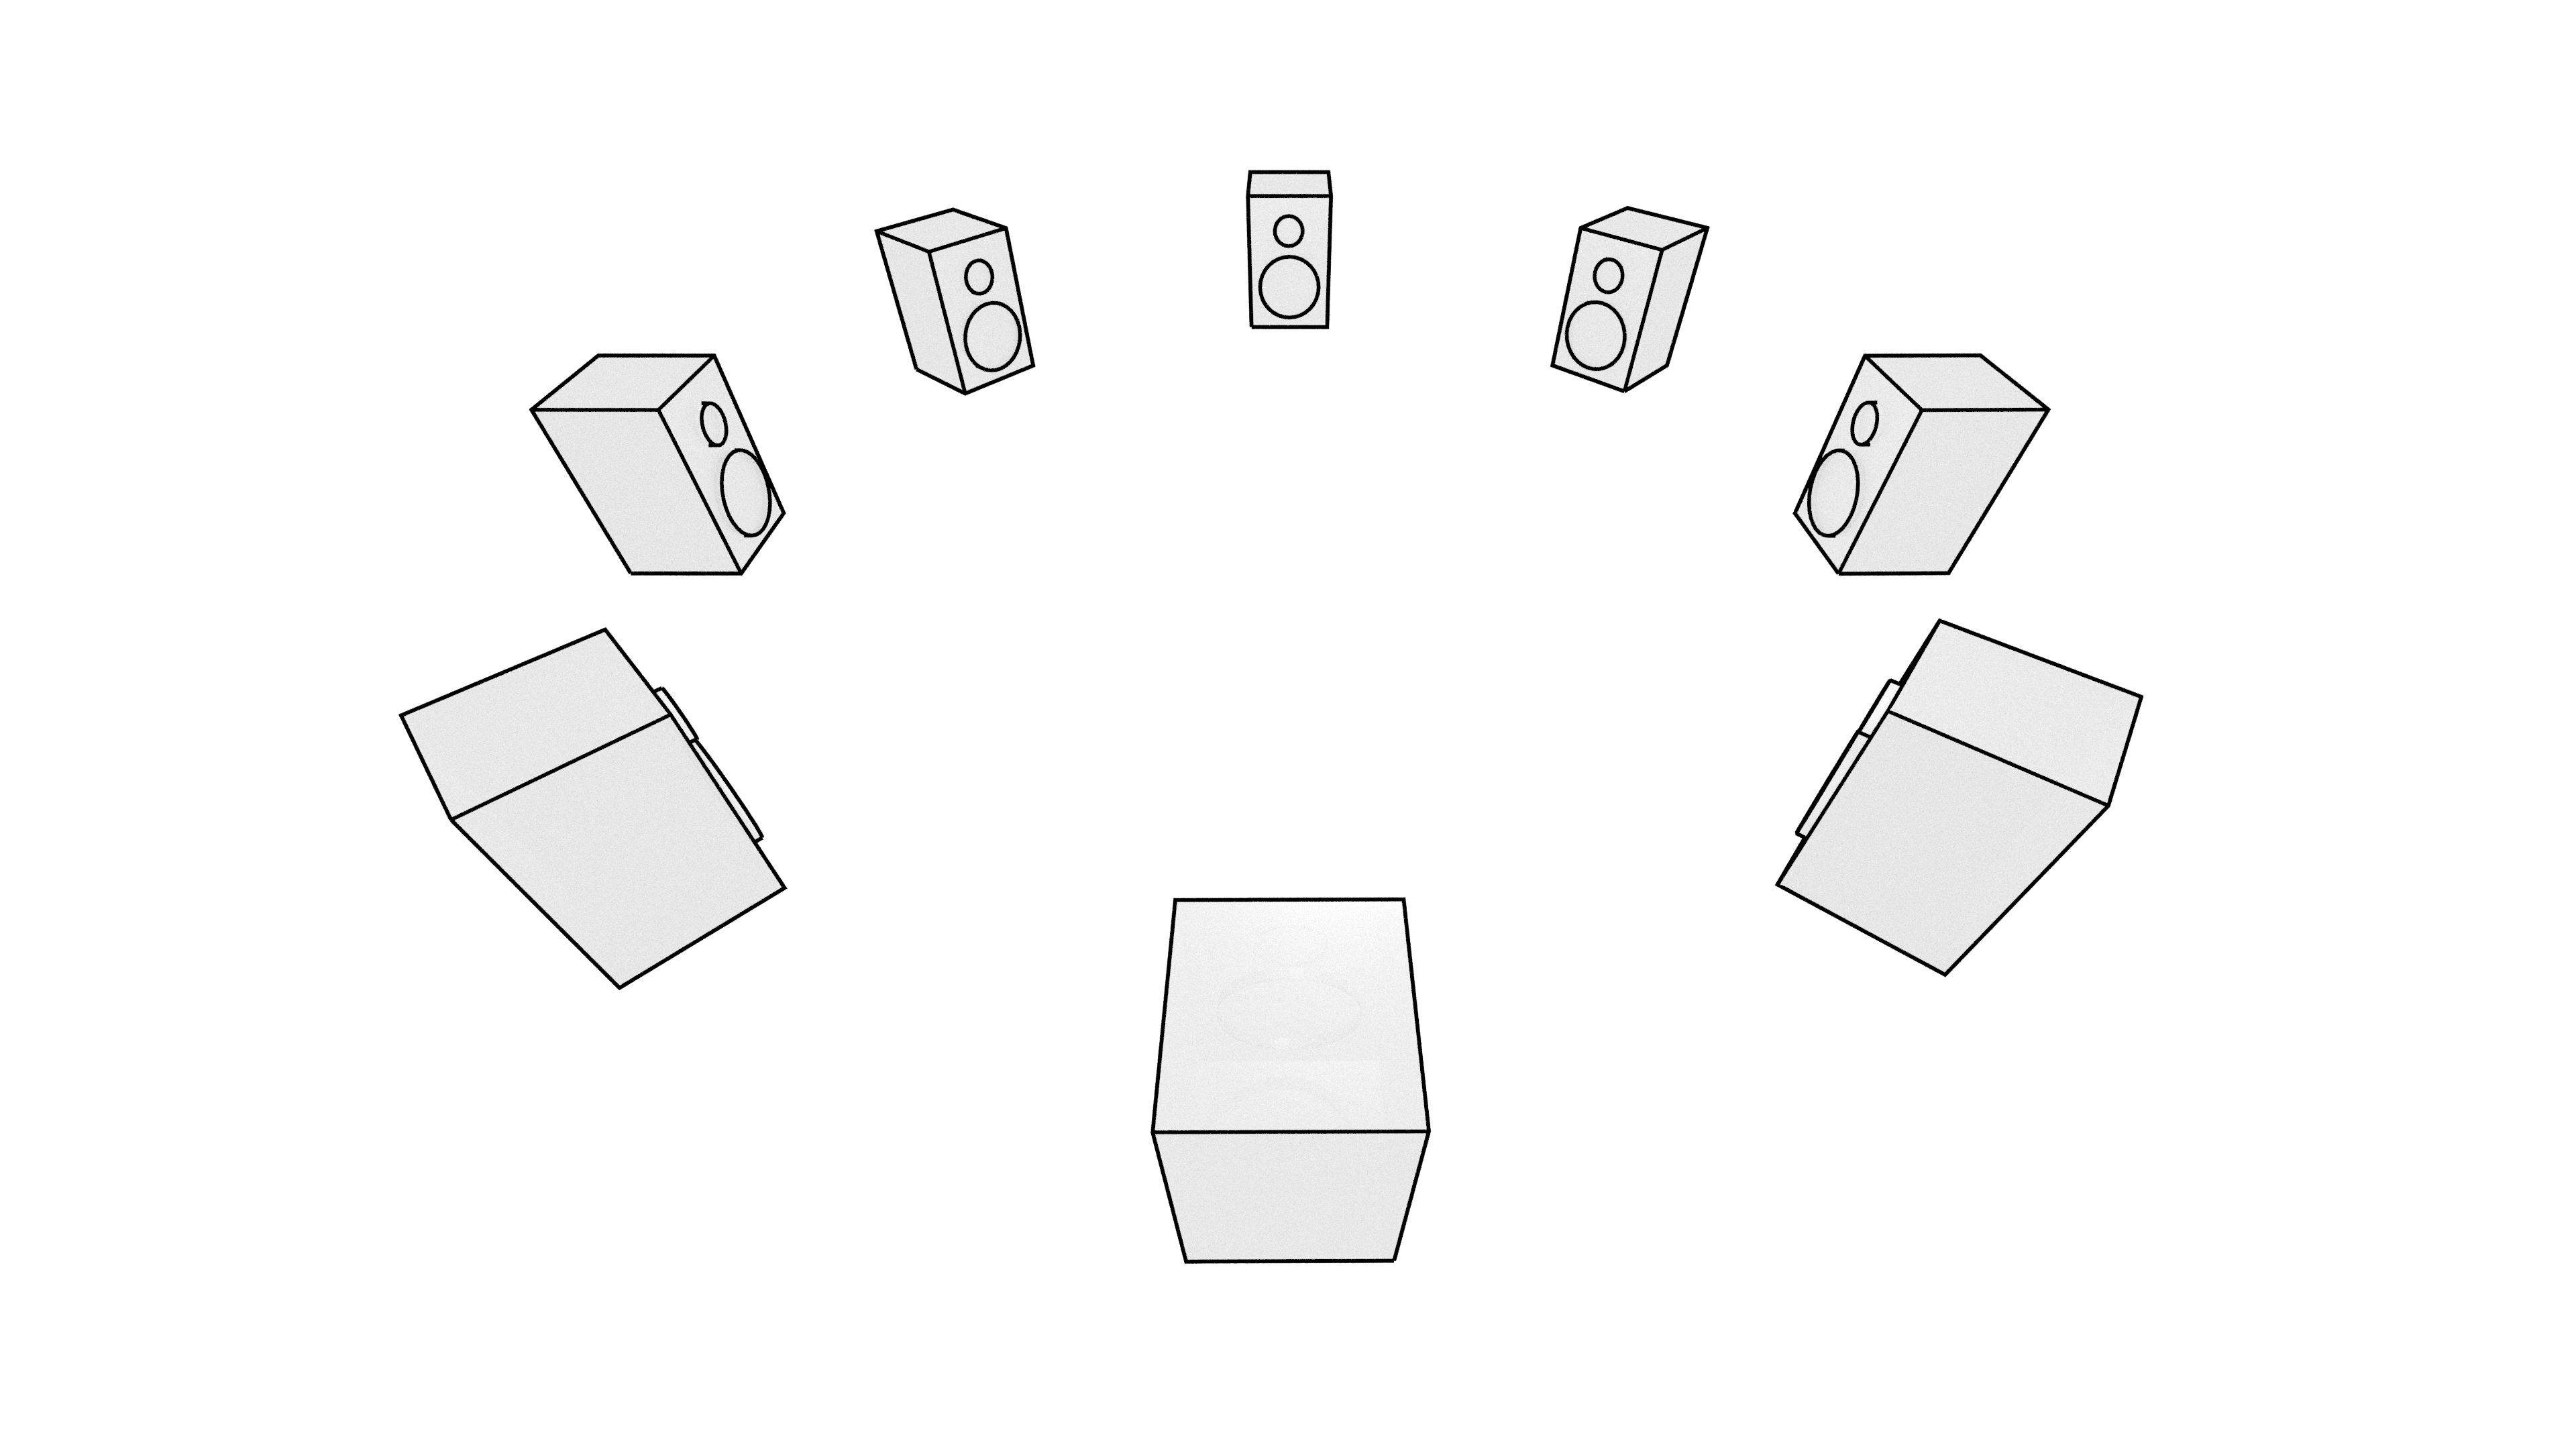
\includegraphics[height=20em]{images/spatial_audio/speaker_array.png}
    \caption{A 2D (horizontal plane) surround speaker array. Image courtesy of the author. \label{fig:speaker_array}}
\end{figure}

\subsection{Decoding to loudspeakers}

The ambisonics panning function $g(\theta)$ 
that yields the power of the signal for a given direction $\theta$ is continuous,
but in case of loudspeaker playback, the sound field must be recreated using a discrete number of point-sources. 
(See \cite{ambisonics_practical_theory} for the definition of $g(\theta)$ and a detailed dive into the math behind ambisonics.)
Only special arrangements of loudspeakers permit direct sampling without introducing undesired
direction-dependant gain variations (as described for first order ambisonics in the previous subsection). 
These so-called \emph{t-designs} are arrangements of speakers where the distance and direction between 
all neighbouring speakers are constant. $t \geq 2N + 1$ loudspeakers 
are required for optimal reproduction of ambisonics of order $N$. \cite{ambisonics_practical_theory}\cite{zotter_all_round_panning_and_decoding}

\paragraph*{Vector Based Amplitude Panning}

To describe some of the more advanced ambisonic decoding techniques, let's first introduce Vector Base Amplitude Panning (VBAP).
First described by Pulkki in 1997 in \cite{pulkki_dsp_tool_vbap_1996} and then in \cite{pulkki_vbap_1997},
VBAP provides a mathematical framework for selecting which loudspeakers from a 2D/3D 
surround arrangement should be activated and with what gains, to reproduce a virtual sound source at a specific direction.

In the simplest example of stereophonic amplitude panning (two speakers positioned in front of the listener),
Pulkki treats the loudspeaker direction vectors as a vector base.
A direction vector for a virtual sound source at an arbitrary point on the arc enclosed by the two loudspeakers
can be calculated as a linear combination of the two basis vectors. The coordinates of the sound source direction vector in that vector space 
are then interpreted as the gain values for each loudspeaker. 
This system is then extended to horizontal arrangements of more than 2 loudspeakers by always activating 
just 2 loudspeakers - the ones that form the arc on which the virtual sound source lies at that moment. 
As Pulkki states, utilising just two loudspeakers at a given time might seem wasteful, but this approach increases 
localisation accuracy. 

The 2D case is then generalised to 3D by utilising triplets of loudspeakers instead of pairs. 
An approach identical to the 2D case is used for arrays of more than 3 speakers.
Picking the correct speaker triplet to activate can however pose a problem in cases 
where the speaker arrangement allows for ambiguous triplet selection and some other situations.
Due to this, VBAP does favour specific speaker arrangements, but it is still a flexible approach 
that can be used in a variety of situations.
\cite{pulkki_vbap_1997}\cite{ambisonics_practical_theory}

\paragraph*{All-Round Ambisonic Decoding (AllRAD)}

The AllRAD approach presented in ``All-Round Ambisonic Panning and Decoding" 
by Franz Zotter and Matthias Frank \cite{zotter_all_round_panning_and_decoding}
combines VBAP and sampling decoders, as described in previous sections, 
to achieve a lower direction-dependant loudness variation and good spatial resolution
while also providing better results on irregular loudspeaker arrangements.

The idea behind AllRAD is first decoding (sampling) the ambisonic signal to a set of virtual speakers 
arranged in a $t$-design, and then using these signals as virtual sources for 
a slightly modified version of VBAP. Decoding to a regular arrangement of virtual loudspeakers
has the advantage of low directional gain variations and good sound localisation, while VBAP
makes this approach usable with real-life non-ideal speaker arrangements
(higher order $t$-design speaker arrays are usually not very practical).

For playback on speaker hemispheres (which are more common than full spheres in practice due to several factors),
as with normal VBAP, one or more imaginary loudspeakers may be added at the bottom of the arrangement,
or at the average direction vector of the real loudspeakers. The signal from the imaginary 
loudspeaker(s) may either be discarded or equally distributed to the neighbouring loudspeakers. 
While this approach does not actually reproduce the direction of sounds coming from below correctly,
it helps avoid the inability to find a matching speaker triplet (which would make these sounds inaudible),
and preserves some of the audio content coming from below (especially for sounds close to the outer ring of the speaker hemisphere).
A similar approach can of course be used for other speaker arrangements where there is no speakers in certain parts of the sphere.
\cite{ambisonic_decoders_slides_stanford}\cite{ambisonics_practical_theory}

I should note that while AllRAD is one of the most flexible and practical solutions available today,
there are multiple other decoding approaches. Overviews of the other approaches can be found in
\cite{ambisonics_practical_theory}, \cite{frank_and_franz_producing_in_ambisonics} and \cite{ambisonic_decoders_slides_stanford}.

\subsection{Decoding to headphones}

Since human listeners can detect directivity cues with just two ears, it stands to reason, that with the right 
technology, 360\degree{} sound can be reproduced on headphones just as well, if not better, than on loudspeaker arrays.
To achieve this, it is required that the main psychoacoustic cues used by humans (as described in section \ref{subsection:spatial_hearing})
are correctly reproduced. Ideally, interaural difference cues
and changes to the frequency composition of the sound induced by the listener's
head and ears need to be accounted for.

\begin{figure}[!ht]
    \centering
    \includegraphics[height=14em]{images/spatial_audio/impulse_response.png}
    \caption{Definition of a delta function and an impulse response. $\delta[n]$ is used to identify the delta function. 
        The impulse response of a linear system is usually denoted by $h[n]$.
        Image sourced from \cite{dsp_book_convolution}. \label{fig:imp_resp_delta_func}}
\end{figure}

All of this can be captured using a so-called Head-related Impulse Response (HRIR).
First, let's figure out what an impulse response is in general. An impulse response is the output of a linear system when a delta function 
(unit impulse) is the input.
Considering a discrete signal ($N$ separate samples of a continuous signal),
a unit impulse is such a signal where the sample at position $0$ has a value of $1$, and all other samples have a value of $0$.
An important property of the delta function is that any signal can be represented as a combination of differently
shifted and scaled delta functions.\cite{dsp_book_convolution}
Figure \ref{fig:imp_resp_delta_func} provides a graphical definition of the delta function (unit impulse) and it's impulse response.
In the case of a HRIR, the impulse response represents how the listener's head and ears affect sound in a so-called free-field 
- an environment with no reflections or reverberations and thus no colouration of sound.\cite{fundamentals_of_binaural_technology}
Of course an ideal free-field environment can not be achieved in practice, but anechoic chambers get sufficiently close.

There are multiple methods and variations of methods of measuring a HRIR; a good in-depth overview can be found in \cite{hrtf_measurement_review}.
The core idea behind most of them is however the same - microphones are placed into the subject's ears, 
a specific sound (an excitation signal) is then played back (often multiple times)
over a loudspeaker located at a specific point in space, and then the impulse response 
of the system is calculated from the recorded audio.
Multiple measurements with the sound coming from different directions and sometimes distances have to be taken.
Often, especially in case of human subjects (as opposed to head models) it is desirable to move the position of the sound source instead of rotating the listener's head. 

In the time domain, the relation between the input and the output of the system is given by the following equation (\cite{dsp_book_convolution}):
\begin{equation}
    y(t) = x(t) * h(t) = \int_{-\infty}^{+\infty} x(\tau)h(t-\tau) d\tau,   
\end{equation}
where $x(t)$ is the input signal, $y(t)$ the output signal, $h(t)$ is the impulse response of the system, 
and $*$ denotes convolution. The same equation can be written for discrete signals as follows~(\cite{dsp_book_convolution}):
\begin{equation}
    y[n] = x[n] * h[n] = \sum_{j=0}^{N-1} h[j]h[n-j],
\end{equation}
for an N-point impulse response $h[n]$ with indexes spanning from $0$ to $N-1$.
Another term that the reader would surely encounter when researching ambisonic decoding to headphones,
and binaural audio in general is a head-related transfer function. A HRTF is nothing more than a HRIR 
in the frequency domain. \cite{fundamentals_of_binaural_technology} Once a HRIR is calculated, 
convolution can be utilised to calculate the response of the system to an arbitrary input signal.\cite{dsp_book_convolution}
Using HRTFs measured at different impulse directions, and utilising interpolation techniques, 
psychoacoustic cues for a sound coming from an arbitrary direction can be reproduced.\cite{hrtf_measurement_review}

Decoding ambisonic audio to headphones using HRTFs can be achieved by utilising virtual loudspeakers.
A decoder such as AllRAD is first used to produce a CBA signal set for some favourable arrangement of loudspeakers, such as a \emph{t}-design, to achieve low loudness variation and good localisation accuracy.
Each of the resulting virtual loudspeaker signals is then convolved with a HRTF measured at an appropriate direction.
Finally, the signals are added together to produce the final binaural mix. \cite{3d_ambisonic_based_binaural_reproduction}

It is worth mentioning that, as with most topics discussed thus far, there are many possible variations and improvements to the base approach. 
Some of them are discussed in \cite{ambisonics_practical_theory}.

\subsection{A comparison of personalised and generic HRTFs}

So-called personalised (or individualised) HRTFs are measured for a specific individual and thus
match how that person perceives sound in everyday life as closely as possible.
Generic HRTFs on the other hand are synthesized from large datasets of individual measurements 
with the aim to provide a good enough experience for most people.
Unsurprisingly, research shows that individualised HRTFs perform better than generic ones, with the main improvement being a reduction in front-to-back confusion.
\cite{localisation_nonindividualized_hrtfs}
However, non-personalised HRTFs show good enough performance in many cases, and are the more common choice in practice due to the 
cost and complexity of measuring individual HRTFs. 
Furthermore, with enough time, a listener's brain is able to adjust to a ``foreign" HRTF - experiments performed in 
\cite{adaptation_to_nonindividualised_hrtfs} show worse localization test performance by inexperienced subjects, 
than those that went through training (both simultaneously hearing a sound and seeing it's position, and trying to determine a sound's position with post-test feedback).
Trained subjects also showed better results when presented with sounds at positions different to the ones used during the training phase of the experiment.

Non-individualised HRTFs are already being widely used in interactive media, especially computer games. 
Sound localisation is important in first-person shooters and similar titles, and plays an enormous role in increasing immersion in VR. 
HRTFs are employed in Overwatch, Counter Strike: Global Offensive, Valorant, and many VR titles. 
There has also been some academic research into the usage of individualised and non-individualised HRTFs in video games.
While \cite{hrtfs_3d_shooter_game} concludes, that individualised HRTFs expectedly showed better localisation performance,
it is of note that the experiment results (Fig. \ref{fig:hrtf_3d_shooter_test_results}) showed a relatively similar horizontal localisation performance between 
(self-reported) experienced players when using non-individualised HRTFs and players using an individualised HRTF. 
This can realistically be attributed to ``expert" players having more experience with other FPS titles with HRTF-based spatial audio, 
as many of the most popular competitive titles do employ it.

\begin{figure}
    \centering
    \includegraphics[width=0.5\textwidth]{images/spatial_audio/hrtf_fps_test_results.png}       
    \caption{Horizontal and vertical localization errors for expert (solid pattern) 
        and casual (hatched pattern) players. Image sourced from \cite{hrtfs_3d_shooter_game}.
        \label{fig:hrtf_3d_shooter_test_results}}
\end{figure}

Another study, that focused specifically on VR games \cite{generic_hrtfs_vr},
showed that sound localisation using generic HRTFs was improved with time, when the players were presented with 
matching visual and auditory stimuli. The improvements didn't occur when no visual stimulus accompanied the sound, 
or when the stimuli were not sufficiently synchronised. The experiments also showed that the improvements in 
localisation didn't transfer to different auditory stimuli (sounds with a significantly different spectral composition).
This however should not pose a problem in case of video games and other hand-crafted experiences,
as they tend to use a comparatively low number of individual sounds, especially 
if only sounds whose accurate localisation is important to the overall experience are taken into account.

%//TODO: mention applied binaural audio somewhere? (apple music spatial audio, etc)

% \cite{blumlein_patent}

\chapter{An overview of spatial audio production software}

\begin{chapterabstract}
    This chapter examines some of the spatial audio production tools
    publicly available at the time of writing and discusses their suitability
    for 360\degree{} video production.
\end{chapterabstract}

\section{DAW-based solutions}

Most tools for producing ambisonic audio come in the form of DAW plugins, most of them in the VST format\footnote{
    VST is a plugin format for digital audio workstations developed by Steinberg Media Technologies. \cite{vst_steinberg}
    While competing plugin formats exist, VST is multiplatform, and one of the most widely supported ones.
}.
They are usually released in the form of plugin suites, consisting of ambisonics encoders (panners) and decoders.

The encoder plugin takes an input (in most cases mono or stereo), computes the spherical harmonic coefficients, 
based on the current panning settings, and outputs an ambisonics representation with the sound placed at the desired direction relative to the listener.
An instance of the encoding plugin has to be placed on each channel that will be used in the final ambisonics mix, as can be seen in figure \ref{fig:encoders_routing}.
Recordings from microphone arrays, and other ambisonic audio can also easily be added to the final mix by simply adding the individual channels together.

\begin{figure}
\centering
    \includegraphics[height=32em]{images/daws_vsts/encoders_setup_cropped.png}       
    \caption{Ambisonic encoder plugins placed on individual channels. Image courtesy of the author. \label{fig:encoders_routing}}
\end{figure}

Using the encoder alone is enough to output an ambisonics mix, but in order for the mixing engineer to hear 
the results of his actions, or to output the mix in CBA format, the ambisonics representation has to be decoded back to channel-based audio.
For these purposes these plugin suites usually include a decoder plugin that converts the ambisonics signals into speaker
feeds for a surround setup, or into a stereo binaural representation using a personalized or generic HRTF.
The decoding plugin is usually placed on the master bus\footnote{A master bus is the final stage in audio processing. It combines the signals from all the individual channels (or tracks) in a DAW or a hardware mixing console.}
- figure \ref{fig:decoder_master}.

\begin{figure}
    \centering
    \includegraphics[height=19em]{images/daws_vsts/master_bus_setup_cropped.png}       
    \caption{A master bus with an ambisonics decoder plugin. Image courtesy of the author. \label{fig:decoder_master}}
\end{figure}

Because the plugin outputs multiple channels of audio, 
the digital audio workstation itself has to provide support for multichannel audio.
The maximum achievable ambisonics order is then limited by three factors - 
available computational power (for real time preview), the plugin itself, and the number of channels supported by 
the DAW. Fortunately, while not prevalent, multi-channel support is present is some of the 
popular digital audio workstations, such as Reaper \cite{reaper_manual} and Pro Tools \cite{protools_manual}; 
Steinberg's Cubase Pro even provides built-in ambisonics support in the form of encoder and decoder plugins, as well as general multi-channel capabilities \cite{cubase_ambisonics}.
Nuendo - another DAW from Steinberg, geared towards industry professionals, provides ambisonics support with advanced features
- their decoder, for example, supports head-tracking to synchronize the audio with head movement (Fig. \ref{fig:nuendo_screenshot}). 
Nuendo also has built-in integration with some game audio middleware systems
\footnote{Middleware systems are software that is integrated into a game engine to handle a specific subset of it's functionality, such as audio playback.}
(Wwise and ADX2), as well as features specific to VR audio
, including support for dearVR Spatial Connect - a virtual reality environment for spatial audio mixing,
which also provides positional data export to the Unity game engine.
\cite{nuendo_features}

\begin{figure}[!ht]
    \centering
    \includegraphics[width=\textwidth]{images/existing_solutions/nuendo_panner_and_head_tracking.png}       
    \caption{Head-tracking and spatial panning in Steinberg's Nuendo.
        Image sourced from \cite{nuendo_screenshot}.
        \label{fig:nuendo_screenshot}}
\end{figure}

Ambisonic plugin suites usually include multiple types of encoders and decoders. 
Various encoders can be used for encoding non-ambisonic content with different directivity patterns, 
e.g. planewave (sound emanating from a single direction) or omnidirectional,
as well as transforming recordings from various microphone arrangements into a standardised ambisonics representation.
Decoders usually differ in their output format - CBA for various speaker arrangements, binaural stereo, etc.

Listed below are some of the more fully featured ambisonics plugin suites (with a bias towards open source).
\begin{itemize}
    \item The Ambisonic Toolkit \cite{ambisonic_toolkit}
    \item ambiX \cite{ambiX}
    \item IEM Plug-in Suite \cite{iem_plugin_suite}
\end{itemize}

The DAW-based approach to spatial audio production provides a lot of flexibility,
especially if working in Reaper or another DAW with similar multichannel and routing capabilities.
The producer is able to use the in-DAW workflows they have grown accustomed to and can benefit
from the vast amount of available plugins. Plugins from different manufacturers, including ambisonic encoders, decoders, 
and spatial effects, can all be used in a single project.
This is approach is popular and flexible, but there is definitely still room for improvement, 
especially for more specialised workflows such as 360\degree{} video production.
One area for improvement is integration between the different software used throughout the production process.
Such functionality is absent from most DAWs, which is to be expected due to the relatively 
low number of users that would benefit from it.
Fortunately, in many cases, such workflows can be improved by plugin developers.

\section{Game Engines}

While digital audio workstations are the obvious choice when it comes to producing any form of audio content, 
including ambisonics, in some cases, other approaches may be more sensible. 
The visual fidelity of modern game engines is already on such a high level, that they can be used for
3D productions. Their object-based audio systems also provide extensive 
functionality including mixing and real time audio processing. \cite{unreal_doc_audio}\cite{unity_manual_audio}
Theoretically, this could allow them to be used as an all-in-one 360\degree{} video production tool.
Unfortunately, in reality, using game engines for 360\degree{} video production might not be a good choice.
Neither of the two most popular commercially available 
game engines provide reliable solutions for exporting 360\degree{} video and audio.

Unreal Engine does come with the ability to export 360\degree{} video out of the box, but only as a series of still
images, and thus without audio. Exporting ambisonics is not supported in any way at the time of writing, 
although workarounds, converting a CBA mix from unreal to ambisonics, can be devised (but quality loss would be inevitable in that case). \cite{unreal_360_export}
Unity doesn't have built-in support for exporting 360\degree{} video or audio, but a third-party solution 
is available.
The "VR Panorama 360 PRO Renderer" tool's Unity Asset Store page \cite{unity_360_export} does claim to support rendering 
360\degree{} video, as well as ambisonics audio ``for YouTube''. But the quality of the implementation and integration with Unity is not guaranteed,
this being a third-party product.

Being able to use a single piece of software
for both the visual and the audio aspects of production is certainly attractive.
Unfortunately, the major commercially available game engines are not currently viable for 360\degree{} video production.
Their feature-set, however, despite being intended for a different use case, 
already provides a great foundation that can be built upon 
by adding some 360\degree{} video specific features.
With the popularisation of spherical video and VR gaming, it is possible that
360\degree{} gameplay demos and game trailers will become more common, and such features will 
be added as demand increases.

\section{3D software}

Studying the manuals for multiple widely adopted 3D software packages
\footnote{Blender, Autodesk Maya, Maxon Cinema 4D, Autodesk 3ds Max, and SideFX Houdini.}
leads to an unsurprising finding - most lack audio features in general, let alone SBA export capabilities.

Both Autodesk's offerings - Maya and 3ds Max provide some degree of audio support, 
but these features are limited and not usable in a spatial audio context. 
Maya's audio support is intended purely for synchronising animation to sound. \cite{maya_manual_audio}
3ds Max does provide a more fully featured audio editing system, but it's limited to arranging pre-rendered CBA clips, 
and is incapable of spatial audio encoding in any form. \cite{3dsmax_manual_audio}

Blender on the other hand does include a spatial sound system.
The user can place speaker objects, representing individual sound sources at arbitrary positions in the 3D scene.
The software allows to choose between several distance fall-off models, adjust the direction in which the sound is emitted 
from each individual speaker object, and even includes doppler effect simulation.~\cite{blender_manual_audio}
The unfortunate part is, that the current version of Blender (at the time of writing - 3.1) only supports exporting stereo.
It is not documented anywhere which technique is used to render this stereo output, but,
based on my listening test\footnote{
    I placed a speaker object directly above a camera moving on the vertical axis, and listened to the result to
    check if there was any height information present.
}, it is not binaural stereo. Interestingly, earlier versions of Blender
(at least up until v2.79\footnote{
    Downloading and launching the aforementioned version of the software confirmed that the feature is present.
})
did include the ability to export 5.1 and 7.1 surround audio, but it has later been removed.
Overall, Blender itself
can also be deemed unusable for spatial audio production.
A Blender add-on which implements OBA export will be mentioned in the next subsection.

There is however an outlier, both in terms of spatial audio support, 
and in terms of the software's general purpose - SideFX's Houdini.
A software with a target audience intersecting those of the previously mentioned programs only to a lesser extent, 
Houdini takes a completely procedural approach to 3D and includes advanced simulation capabilities.
Audio simulation capabilities are also present, and ``simulation" is truly the correct word to use here.
Houdini's spatial audio system supports distance fall-off, doppler effect, and even obstacle interference,
including per-obstacle customisation of transmission and absorption levels for different frequencies.~\cite{houdini_spatial_chop}\cite{houdini_acoustic_chop}
As in Blender, sound objects with customisable emission direction can be placed in the 3D scene. \cite{houdini_sound_object}
The sound can then be ``captured'' by an arbitrary amount of virtual microphone objects \cite{houdini_microphone_object}, effectively allowing
to record audio using microphone setups analogous to those used in the real-world, which makes ambisonics and CBA recordings possible.
While I could not find any examples of spatial audio rendered using Houdini, and thus can not assess the quality of the output,
the capabilities of this solution seem vast.
Houdini, however, is not an audio production environment. Using it's spatial audio system, as with it's other aspects,
requires much more specialised knowledge than using other approaches, such as DAWs and game engines.

\section{Other solutions}

This section includes some interesting solutions that didn't fall into any of the above categories 
and don't have alternatives that would warrant adding a separate subsection. 
% Some of them are not strictly related to 360\degree{} video production, but I still felt their 
% inclusion would benefit the reader in terms of providing a broader overview of the spatial audio field.

\paragraph*{IRCAM Panoramix}
Designed and developed at IRCAM
(French: Institut de recherche et coordination acoustique/musique, English: Institute for Research and Coordination in Acoustics/Music), 
Panoramix is a post-production and mixing workstation for 3D-audio content. 
It aims to provide a 
``comprehensive environment for mixing, reverberating, and spatializing sound materials from different microphone systems:
surround microphone trees, spot microphones, ambient miking, Higher Order Ambisonics capture.''
(\cite{panoramix_conference_paper})
It is not meant to replace a digital audio workstation, but rather work in conjunction with one, 
aiding in the mixing stage of the production workflow. 
The design is inspired by hardware mixing decks with each track represented by a vertical strip. 
There are various types of input tracks, accommodating different input signal types, e.g. mono, ambisonic, different microphone arrangements.
It also includes various other tools useful in spatial mixing and mastering, such as a reverberation engine, 
as well as the usual mixing instruments - an equaliser and a compressor/expander. 
A concise feature list can be found in \cite{panoramix_ircam_website}; a conference paper (\cite{panoramix_conference_paper}),
that delves deeper into the motivation behind creating the software
and the design decisions made in the process might also be of interest to the reader.

\paragraph*{The ``soundobjects'' Blender add-on}
Created by Jamie Hardt (@luvcapra on GitHub), ``soundobjects'' is a Blender add-on
that allows export of OBA in the ADM Broadcast WAV format. (See \cite{dolby_adm_spec} for the format specification.)
It provides Blender operators that allow to import WAV audio files, add speaker objects to existing objects in the scene, assign audio files to them, 
and export a file in the ADM Broadcast-WAV format where each audio object corresponds to a Blender speaker object in the scene.
The resulting file contains a sound object for each of the speaker objects in the blender scene.

Unfortunately, it seems this project is no longer being developed or maintained. 
The last commit in the project's GitHub repository (\cite{soundobjects_addon_repo}) adds a note 
about changes in ProTools that result in the inability to import WAV files produced by the add-on.
Despite this, the project is still an interesting tool, and, with interest from the open source community, 
could be revitalised and improved.

% \section{Summary}
% Of all the approaches presented in this sections, the ecosystem around producing ambisonics using 
% digital audio workstations seems to be the most evolved. 
% Since manipulation and creation of 
% audio content is the sole purpose of DAWs, it is unsurprising that the software is being adapted for spatial audio.
% While other approaches should still be considered depending on the task at hand,
% the versatility and extensibility provided by a DAW-based spatial audio production workflow 
% makes it the clear winner for producing
% // TODO: maybe add summary section if there's time


\chapter{UI/UX Design}\label{chapter:ui_ux_design_reqs}

\begin{chapterabstract}
    This chapter explains the reasoning behind some of the core design decisions, 
    specifies the software requirements, 
    and provides an overview of the GUI layout.
\end{chapterabstract}

\section{Real-time approach}
Ambilink's\footnote{``Ambilink'' is the name given to the software during early stages of development.} main goal lies in allowing to utilise animation data 
from a Blender scene for ambisonic panning in a DAW. This is achieved with a pair of plugins - a Blender plugin and a VST plugin.
The Blender plugin (or ``add-on'', using Blender's official terminology) 
provides data about the 3D scene to instances of the VST plugin, that perform the ambisonic panning.
Deciding how this data will be passed from the Blender add-on to the VST was the earliest design decision that had to be made, 
since the chosen approach would dramatically affect the way the software functions, and, naturally, the user experience. 

One solution would be to export animation data from Blender to a file.
The data could then be imported by the VST plugin.
Unfortunately, such a solution, although simple to implement, would be quite suboptimal from a UX perspective.
Music production experience has taught me that immediate feedback is immensely helpful when making creative decisions, 
and that decisions made by sound designers and mixing engineers are undoubtedly of creative nature.
Thus, from the very beginning, I've designed the software to include real-time preview functionality - 
the panning directions are continuously updated based on the current state of the Blender scene, 
allowing the user to immediately hear how adjustments performed in Blender affect the audio mix.

Of course, the real-time approach also has it's downsides. It increases the overall complexity of the system,
and may introduce new types of problems stemming from connection issues. 
Communication latency may also negatively affect responsiveness.
A good implementation should however be able to avoid or mitigate these flaws.

\section{Requirement definition}
Once the decision to make the system real-time was made, I've settled on some functional and non-functional requirements to guide the development.
\subsection*{Functional requirements}
\begin{funcreqs}
    \item The system consists of two components - the Blender add-on and the VST plugin.
    \item The user is able to pick an object from the Blender scene using the VST plugin.
    The location of that object is then used to calculate the panning direction used by the VST plugin.
    \item Whenever the location of a Blender object is updated (manually or during animation playback), 
    the panning directions are updated in real time. (Communication between the two components is performed in real time.)
    \item When a VST instance is bound (subscribed) to a specific Blender object, renaming or deleting the object in Blender is reflected by the VST GUI.
    \item The VST plugin supports offline rendering\footnote{Offline rendering refers to exporting the audio, as opposed to real-time (online) playback during the production process.}.
    The exported audio is synchronised to the animation.
    \item The distance from a Blender object to the camera affects the gain of the respective VST distance; 
    the user is able to choose from multiple distance attenuation models.
    \item The user is able to pick the Ambisonics order and normalisation type (N3D or SN3D) used by the plugin.
\end{funcreqs}

\subsection*{Non-functional requirements}
It has to be noted that since the software can run on any number of hardware configurations,
it is hard to define performance-related requirements unambiguously. 
Thus, the ``scales well'' formulation used in the non-functional requirements below
should be understood as ``scales well for the hardware''.

\begin{nonfuncreqs}
    \item Selecting an object from the Blender scene via the VST GUI is quick,
    even when the scene contains a large number of objects.
    \item Real-time direction updates have an acceptable delay, ideally less than 0.5 seconds.
    \item The system scales well for Blender scenes containing a large number of objects (e.g. thousands). 
\end{nonfuncreqs}

\section{User interaction}
% Suggested: nejaky use-case diagram?? -> Would not bring value, single actor, single use case, functional requirements specified differently
With the requirements in place, the next step was designing the way the user will interact with the software.
In case of Ambilink, this was a relatively straightforward process, 
since the system has a single use case, that only requires limited user interaction.
A user's workflow might roughly follow these steps:
\begin{enumerate}
    \item Open the Blender project, and start the Ambilink Blender add-on.
    \item Open the DAW, and place the Ambilink VST on the channels containing sounds that should correspond to objects in the Blender scene.
    \item For each instance of the Ambilink VST, select an object from the Blender scene.
    \item Adjust ambisonics-related settings (order, normalisation type) to match what's being used in the project.
    % //TODO: if there's time and it's easy to implement, store these "global" settings in a config file. Otherwise, add a note about this being a limitation of the current version.
    \item Make any necessary adjustments to the Blender scene, or the audio mix, including adjusting distance attenuation parameters of the Ambilink VST.
    \item Render the resulting audio.
\end{enumerate}

\subsection{Blender add-on}
The Blender plugin needs to support two main actions - launching and stopping the server that will provide data to the VSTs.
Most operations in Blender are realised using so-called operators that essentially encapsulate any action that can be performed by the user.
Operators can be invoked via buttons in the GUI or using Blender's search functionality.
Because the user shouldn't have to start or stop the server often, I've chosen to avoid adding an additional panel to the GUI.
Instead both actions are realised using operators that can be invoked from the \cppinline{File > Export} menu, or using search.

The Blender add-on depends on an external Python module.\footnote{External dependencies will be discussed in Chapter \ref{chapter:implementation}.}
I did not want to include the module's code as part of the addon, or to automatically install third-party modules without informing the user.
Instead I've chosen to be transparent and require the user to explicitly initiate dependency installation.
This can be done by pressing a button in Ambilink's add-on preferences panel which can be accessed through Blender's preferences dialogue.
If dependencies aren't installed and the user invokes the ``Start Server For Ambilink VST'' operator,
an error message is shown that instructs the user to install dependencies via add-on settings.

\subsection{VST plugin}

The VST plugin should allow the user to perform a much wider range of actions - selecting an object from the Blender scene, changing distance attenuation and ambisonics parameters.
Figure \ref{fig:gui_prototype} shows a wireframe of the user interface created before implementation.
The GUI consists of a main screen that is shown at launch and two additional screens - the object selection screen and the settings screen.

\paragraph*{Main screen}
The main screen displays the currently active object (if any), and a visual indicator of the current direction from the camera to the object.
It also allows to adjust the distance attenuation type and maximum distance to the camera at which the sound gain will be above 0 dB.
The distance attenuation parameters are located on the main screen to minimise the number of clicks required to adjust them. 
This is done because various sounds may require different values, 
depending on the distance at which the user would want them to become audible.
By pressing the button on the right side of the active object indicator the user can transition to the object selection screen.
The settings screen can be accessed by pressing the ``Settings'' button located in the top right corner of the UI.

\paragraph*{Object selection screen}
The object selection screen allows the user to select an object from the Blender scene. Since the Blender scene may include a 
high number of objects, a search box is present in the top part of the UI, allowing the user to quickly find a specific object.
When searching, the first object in the list is highlighted; the user can then select that object by pressing the ``Enter'' key.

\paragraph*{Settings screen}
The settings screen is reserved for plugin parameters that are not expected to be adjusted often,
and can thus be placed on a separate screen to avoid cluttering the main UI (and save space for adding new parameters further down the line).
Right now it only includes the ambisonics order and the normalisation method.
The user should only need to adjust these parameters once per project most of the time.

\begin{figure}    
    \includegraphics[width=0.9\textwidth]{images/implementation/gui_wireframe_whitespace_bottom.png}
    \centering
    \caption{Prototype GUI layout for the VST plugin. From top to bottom: main screen, object selection screen, settings screen.
             Image courtesy of the author. \label{fig:gui_prototype}}
\end{figure}

% ===========================================================
% ===================== IMPLEMENTATION ======================
% ===========================================================
% - IPC Communication Overview (mentions NNG, and it's role)
% - VST Plugin
%   - Technologies Used
%   - High level structural overview
%   - IPC Client
%   - Encoder
%   - Passing data lock-free (prilohy)
% - Blender Plugin
%   - Technologies Used
%   - Structural overview
%   - Overcoming Blender API Limitations (prilohy)

\chapter{Implementation}\label{chapter:implementation}

\begin{chapterabstract}
    This chapter provides an overview of the implementation of the Blender add-on and the VST plugin.
    It present the structure of the IPC protocol, describes the top level architecture of each component, 
    and provides some insight into the challenges that had to be solved.
\end{chapterabstract}

\begin{figure}[!h]
    \includegraphics[width=\textwidth]{images/implementation/plugin_interaction_diagram.png}
    \caption{Diagram of high level interaction between the VST instances and the Blender plugin.
        Image courtesy of the author. \label{fig:component_diagram}}
\end{figure}

\section{IPC Protocol}
To minimise latency in communication between the Blender add-on and the VST plugin, Ambilink utilises IPC
\footnote{IPC is a generic term - interprocess communication may very well be realised using TCP or other network protocols.
In the context of this thesis, however, the term IPC is used to refer to any form of ``direct'' interprocess communication, such as named pipes or shared memory.}.
Since Ambilink is developed in a way that should enable eventual support of all three major operating systems,
utilising OS-specific IPC mechanisms directly was undesirable.
Instead, I've chosen to entrust the low level details of interprocess communication to a third-party library - NNG (nanomsg-next-gen).
NNG is multiplatform, provides support for various transports (e.g. IPC, TCP, WebSockets), as well as common communication patterns (e.g. Request/Response, Publisher/Subscriber).
While NNG itself is written in C, wrappers exist for many popular programming languages, including Pynng for Python, as well as nngpp for C++.
(The latter serves more as a quality of life improvement, as NNG's C interface can of course be used directly from C++ code.)
Using the library also highly increases flexibility of the implementation, allowing, for example, to replace IPC with network communication via TCP or WebSockets with minimal effort.
All of this made NNG a great choice for Ambilink.

Figure \ref{fig:component_diagram} illustrates how the individual components are connected via IPC from a high level perspective.
The Blender plugin takes on the role of a server, providing information about the Blender scene to
an arbitrary number of clients - instances of the VST plugin. 

\begin{figure}
    \centering
    \includegraphics[width=0.95\textwidth]{images/implementation/basic_comm_sequence.png}
    \caption{Communication sequence between the Blender plugin and an instance of the VST plugin during real-time (online) rendering.
             Messages with the suffix ``request'' or ``reply'' are sent using Req/Rep.
             Messages with the suffix ``msg'' are sent using Pub/Sub.
             Image courtesy of the author. \label{fig:basic_comm_sequence}}
\end{figure}

A sequence diagram illustrating communication between the two plugins in real-time rendering mode is shown in figure \ref{fig:basic_comm_sequence}.
First, the user picks an object from the Blender scene. The VST instance then subscribes to that object,
requesting the Blender add-on to begin informing it about updates to the object's location and other important events.
The object is then renamed in Blender, and a rename notification is published by the Blender add-on, allowing the VST GUI to update the object name.
Finally, the VST instance is deleted by the user; it's destructor sends a request to unsubscribe from the object. 
(Object position updates would have continued after the rename message if the instance hadn't been destroyed.)
Two different communication patterns implemented by the NNG library were used during that sequence:
\begin{description}
    \item[Request/Reply (Req/Rep)] This pattern is used for all communication initiated by the VST instance - requesting the list of objects in the Blender scene, subscribing to an object, 
    requesting object location data for offline rendering, etc.
    \item[Publisher/Subscriber (Pub/Sub)] In this pattern, a single publisher produces messages that are consumed by multiple subscribers.
    Ambilink starts using this pattern once a VST instance is subscribed to an object. The Blender plugin serves as the publisher, and the VST plugin instances as the subscribers.
    Messages published by the Blender plugin include object location updates (published multiple times per second for all objects with at least one subscribed VST instance),
    object name updates, and object deletion notifications.
\end{description}

\subsection{Protocol messages}
\begin{listing}[ht]
    \begin{minted}{python}
    class ReqRepCommand(IntEnum):
        OBJ_LIST = 0x01
        OBJ_SUB = 0x02
        OBJ_UNSUB = 0x03
        PREPARE_TO_RENDER = 0x04
        INFORM_RENDER_FINISHED = 0x05
        GET_RENDERING_LOCATION_DATA = 0x06
        GET_ANIMATION_INFO = 0x07
        PING = 0xFF
    
    class ReqRepStatusCode(IntEnum):
        SUCCESS = 0x00
        OBJECT_NOT_FOUND = 0x01
        INVALID_REQUEST_DATA = 0x02
        INTERNAL_ERROR = 0xFE
        UNKNOWN_COMMAND = 0xFF
    \end{minted}
    \caption{Definition of IPC protocol constants used in Req/Rep messages. (From the source code of the Blender add-on.)}
    \label{code:ipc_constant_definition}
\end{listing}

This section provides an overview of the message structure for each communication patter used in the IPC protocol. 
The \cppinline{documentation/ipc.md} file included on the attached media defines the structure of 
each individual message type. Alternatively, documentation generated using Doxygen (\cppinline{documentation/Doxyfile} on the attached media) 
will also include the contents of the file.

\paragraph*{Request/Reply}
The Request/Reply part of the  protocol consists of a set of commands differentiated by a single-byte command code.
A request always starts with the command code, and a reply starts with a status code (also a single byte) indicating if the operation was successful
or the reason it failed. In both cases optional command-specific data may follow. 
Listing \ref{code:ipc_constant_definition} shows the list of all commands and status codes and the corresponding constants.

\paragraph*{Ambilink IDs}
During the initial stage of communication (before a subscription is established) Blender objects are referenced by their name.
While object names in Blender are unique, using the object's name as the identifier would not be viable as the objects 
can be renamed after the subscription is established.
It would also be inefficient - a whole string would have to be passed for every request referencing a specific object,
as well as in every message published by the Blender add-on, increasing the size of most messages.
Because of these factors, once a subscription is established, a unique numeric identifier is used to reference Blender objects.
This value, called an Ambilink ID, is assigned by the Blender plugin
\footnote{The process of Ambilink ID assignment will be discussed in more detail in \ref{subsection:blender_api_fun}.},
and returned as part of the reply to an \cppinline{OBJ_SUB} request.

\paragraph*{Publisher/Subscriber}
Messages published by the Blender add-on start with the AmbilinkID of the object they relate to.
This allows each VST instance to filter out irrelevant messages based on the first two bytes.
After the Ambilink ID, a single-byte message type identifier follows. The Blender add-on publishes the following message types:
\cppinline{OBJ_POSITION_UPDATED}, \cppinline{OBJ_RENAMED}, \cppinline{OBJ_DELETED}. 
\cppinline{OBJ_POSITION_UPDATED} messages include the location of the object in camera space. 
Using camera space coordinates allows to reduce the bandwidth consumed by these messages 
since only one set of coordinates needs to be transmitted. The direction and distance from the object
to the camera are then calculated by the VST plugin.

\subsection{Offline rendering}

\begin{figure}
    \centering
    \includegraphics[width=0.9\textwidth]{images/implementation/offline_render_comm_sequence.png}
    \caption{Sequence diagram illustrating communication in offline rendering mode.
             Image courtesy of the author. \label{fig:render_comm_sequence}}
\end{figure}

As can be seen from the sequence diagram in figure~\ref{fig:render_comm_sequence}, 
communication during offline rendering (when the audio is being rendered to a file) significantly differs from communication during real-time playback.
Pub/Sub is not used, instead, every interaction is initiated by the VST.
The \cppinline{PREPARE_TO_RENDER} request includes no additional data and serves as a notification for the Blender plugin 
that a render is about to begin. The Blender plugin will receive this message from each VST instance,
but only the first one will have an effect. While this may seem wasteful, it greatly simplifies the protocol.
Otherwise, all the VST instances would have to communicate with each other, agreeing on a single ``master'' instance.
Once a \cppinline{PREPARE_TO_RENDER} message is received, the Blender plugins stops publishing \cppinline{OBJ_POSITION_UPDATED} messages until the render ends, and invalidates
the cache used during the previous offline render.

To render the audio, a VST instance needs to know the object's camera space coordinates at each frame of the animation.
Instead of requesting all the animation data at once, the VSTs first request the number of frames and FPS of the animation, 
and then get the data in slices using multiple \cppinline{GET_RENDERING_LOCATION_DATA} requests.
(Denoted in fig. \ref{fig:render_comm_sequence} by the ``loop'' fragment.)
This is done because the DAW's GUI thread might be blocked until the first audio sample buffer is processed.
\footnote{This is the case for at least one DAW - Reaper.}
Since Ambilink would not have been able to process the first buffer until all the rendering data is received,
such an implementation would have made the GUI of some DAW's unresponsive for unacceptable periods
when entering rendering mode. Getting rendering data in slices also allows audio processing and IPC to be performed in parallel.

Because the animation may be very long, there is a limit to the number of slices held in memory by each VST instance.
If the memory limit is reached, the VST instance waits for the audio thread to consume the previous slice 
of location data before fetching the next one.

\section{VST plugin}\label{section:vst}
The Ambilink audio plugin is developed in C++ using the JUCE framework and targets Steinberg's VST3 interface\footnote{
    Since VST3 is the only version of the interface that is currently supported by Steinberg,
    I've been mostly referring to it as ``VST'' up to this point and will continue to do so
    unless differences between versions of the standard are discussed.
}. It outputs ambisonics up to fifth order
(The reasons behind this limitation are described in \ref{subsection:vst_limitations}.)
with ACN channel ordering and N3D or SN3D normalisation (configurable via the settings screen).
The code base is multiplatform, but, at the time of writing this thesis, the build system is only operational on Linux.
Documentation comments are used throughout the code base; documentation can be generated using Doxygen 
(see \cppinline{documentation/Doxyfile} on attached media).

\subsection{Third-party libraries}
While developing a VST plugin without a specialised framework is possible, it is highly time consuming,
and takes a lot of ``reinventing the wheel'', that's why Ambilink uses JUCE.
It provides all of the base functionality required for building audio plugins
- a relatively convenient wrapper on top of the base VST interface, a GUI system,
 audio processing primitives, as well as other features not as pertinent to this specific project.
Developing the Ambilink VST with JUCE also opens the opportunity to provide the plugin in other formats 
later on without requiring major changes to the codebase.
Another important factor is that the JUCE framework has a large user base, increasing the number
and availability of learning resources, which was of great help, since I had no prior experience developing audio processing plugins.
Finally, it is dual-licensed under GPLv3 and a proprietary commercial license,
enabling it's use in this project. Besides JUCE, the VST plugin component also uses the Spatial Audio Framework (\cite{saf_repo}) to calculate the spherical harmonics coefficients for a given direction of sound,
as well as vector data types and some useful trigonometric functions from GLM (\cite{glm_repo}).

\subsection{Software architecture}
An audio plugin written with JUCE consists of two main parts. An \cppinline{AudioProcessor} class 
deriving from the \cppinline{juce::AudioProcessor} virtual base class that performs the actual audio processing,
receives audio, MIDI, and other data from the host software. 
The plugin's GUI is implemented in the \cppinline{AudioProcessorEditor}
class that derives from \cppinline{juce::AudioProcessorEditor}.
An instance of the \cppinline{AudioProcessor} class always exists while the plugin is loaded.
\cppinline{AudioProcessorEditor}, on the other hand, is only instantiated once the plugin's GUI editor is open, and is
usually\footnote{Such details may differ between different DAWs.}
destroyed as soon as it is closed.\footnote{A VST plugin does not require a custom GUI, DAW's implement a default GUI for the various audio parameters defined by the VST interface. This was not a viable option for Ambilink.}

\begin{figure}%[!ht]
    \centering
    \includegraphics[width=0.7\textwidth]{images/implementation/vst_simplified_class_diagram.png}
    \caption{Simplified class diagram for the Ambilink VST plugin. (This diagram only includes the most important classes, and is not by any means an exhaustive representation of the whole architecture.)
    Image courtesy of the author. \label{fig:vst_class_diagram}}
\end{figure}

Figure \ref{fig:vst_class_diagram} shows the high level structure of the Ambilink VST plugin.
The \cppinline{AudioProcessor} class holds instances of the \cppinline{IPCClient} and the \cppinline{BasicEncoder} classes.
The \cppinline{IPCClient} class handles communication with the Blender plugin, and the \cppinline{BasicEncoder} class performs the 
ambisonic panning. (The two classes have no knowledge of each other, the direction data is passed through the \cppinline{AudioProcessor} class.)

\subsection{IPC}
The \cppinline{IPCClient} class is implemented as a state machine. The states and transitions can be seen in figure \ref{fig:ipc_state_machine}.
The ``Error'' state and corresponding transitions, as well as transitions to the ``Disconnected`` state are omitted from the diagram to keep it comprehensible.
Whenever connection to the Blender plugin is lost (e.g. if Blender is closed, or the server is stopped by the user), 
the IPC client transitions to the ``Disconnected'' state, regardless of what state it was in previously.
Whenever an exception not caused by connection loss occurs in any of the states, the VST transitions to a special ``Error'' state. 
The GUI then displays an error message, and a button allowing to transition back to the ``Disconnected'' state.
(The plugin will then automatically transition to either ``Connected'' or ``Subscribed'', depending on what state it was in before the error occurred.)
While the users should hopefully never be able to experience the error screen by themselves,
having such a fail-safe allows the plugin to recover gracefully from situations that would have otherwise lead to a crash.

\begin{figure}%[!ht]
    \includegraphics[width=0.8\textwidth]{images/implementation/vst_ipc_state_machine.png}
    \centering
    \caption{State machine diagram describing the way IPC is implemented on the VST side.
             Image courtesy of the author. \label{fig:ipc_state_machine}}
\end{figure}

\cppinline{IPCClient} spawns two threads, one for each communication pattern - a requestor thread, and a subscriber thread.
Each class implementing a state has specific functions to send requests to the Blender plugin,
and to receive messages published using Pub/Sub.
These functions are called by the main \cppinline{IPCClient} class from the respective threads.

To reduce coupling, other parts of the plugin control IPC using a custom event system.
For example, the \cppinline{ObjectSelectionScreen} class can instruct the \cppinline{IPCClient} to subscribe to an object by publishing an event.
The event is passed to \cppinline{IPCClient} through the \cppinline{AudioProcessorEditor} and \cppinline{AudioProcessor} classes.
This is done to further reduce coupling and allow some events to be ``intercepted'' and acted upon by classes other than the \cppinline{IPCClient}.

Once an event reaches the \cppinline{IPCClient}, it is added to a lock-free queue implemented using atomic variables (The implementation used in Ambilink is inspired by Fabian Renn-Giles's \nobreak{farbot} library \cite{farbot_repo}.).
Thread-safety is required since the events are added and removed by different threads; the lock-free implementation reduces overhead of posting an event.
\cppinline{IPCClient}'s requestor thread consumes events from the queue, and passes them to the currently active state,
the state class can then perform any required action, e.g. sending requests or initiating a transition to a different IPC state.

Upon transitioning to the ``Subscribed'' state, the subscriber thread is spawned and begins consuming messages published by the Blender plugin.
When an \cppinline{OBJ_POSITION_UPDATED} message is received, it calculates the direction and distance to the object from the camera space coordinates, 
and updates the values of atomic variables, that are then read by the audio thread and passed to the encoder. 

\subsection{Multithreading in a real-time context}
Real-time audio processing is quite different from most problems usually encountered by programmers.
In case of VST plugins, the host software manages the high-priority threads used for audio processing.
The plugin's processing function (\cppinline{AudioProcessor::processBlock()} in case of plugins using JUCE) is repeatedly called from the audio thread,
each time with new audio and/or MIDI data for the plugin to process. \cite{juce_audioprocessor_doc}
The main caveat is that this callback has to always finish in time. Any delay, even if it occurs extremely rarely
will result in audible artifacts in the audio. \cite{rt_101_talk_part_1}\cite{locks_in_real_time_blog_post}

For example, if the sample rate of the host software is $44.1kHz$, and the size of the audio buffers passed to the plugin is 128 samples,
then the \cppinline{AudioProcessor::processBlock()} function must take less than $(1/44100)*128 = 0.0029s$ to execute, which is just under $3ms$\footnote{
    The sample rate can be significantly higher (usually in the range of $44.1-192 kHz$). Buffer sizes can go down to 32, or even 16 samples. (Speaking from personal experience using DAWs and working with audio.)
}. \cite{locks_in_real_time_blog_post}
This limitation rules out any operation that doesn't have a reliable time limit.
Examples of such operations include accessing files, any form of network communication (or IPC), and, importantly,
using mutex-based thread synchronisation techniques.
Practically any call to a function not implemented by the program should be treated as not real-time safe
unless the documentation explicitly states otherwise. \cite{rt_101_talk_part_1} 
All of these operations can of course be performed on other threads, but if the data needs to be passed to the audio thread
it has to be done without using traditional synchronisation primitives.
Thankfully, even when using locks is out of the question, race conditions can be avoided with good design and some tricks.
In simpler cases, using an atomic value that is modified by one thread and read by another is sufficient, 
but various thread-safe lock-free data structures, such as single consumer single producer FIFO queues can also be implemented (mostly by clever use of atomic variables).
For further information on real-time audio programming I would recommend the two part talk by Fabian Renn-Giles and Dave Rowland \cite{rt_101_talk_part_1}\cite{rt_101_talk_part_2},
which I used as the main source of information on this topic.
Fabian Renn-Giles's open source farbot library \cite{farbot_repo} which implements many real-time safe data structures may also be of interest to the reader.

In case of Ambilink, the data used in the audio processing callback has to be passed from the Pub/Sub thread.
Since the data is small\footnote{
    A struct of two \cppinline{float}s for the direction and a single \cppinline{float} for the distance.
}, 
this is realised using a pair of atomic variables that are ensured to be lock-free
by static assertions (\cppinline{std::atomic<T>::is_always_lock_free}). The atomic variables are stored by 
\cppinline{IPCClient} and read by the audio thread whenever required.
In offline rendering mode, however, a lock is utilised so the audio thread can get access 
to the instance of the \cppinline{OfflineRendering} state\footnote{
    The mutex is only used to prevent the \cppinline{IPCClient} from switching to a different state,
    which would result in destruction of the \cppinline{OfflineRendering} object.
    Synchronisation between the Req/Rep thread and the audio thread,
    once the audio thread does gets access to the state, is performed using 
    atomic variables.
}. This does not really pose a problem since the audio 
is not played back in real time in this case and because locking the mutex
will be uncontested unless a communication error occurs and IPC needs to switch to a different state.
It is however undebatable that this part of the implementation could benefit from optimisation in the future.

\subsection{Encoder}
As mentioned previously, \cppinline{BasicEncoder} is the class that handles ambisonic panning of the incoming audio. 
On each invocation of the \cppinline{AudioProcessor::processBlock()} function, the encoder's 
direction and distance parameters are updated. In real-time mode, the latest value processed by the \cppinline{IPCClient} is used.
In offline rendering mode, direction and location at the respective time in the animation are used.

\begin{listing}[ht]
\begin{minted}{python}
def encode(input_buffer, ambisonic_order, direction, distance, 
           max_distance, distance_attenuation_curve)
{
    curr_sh_coefficients = 
        calc_spherical_harmonic_coefficients(ambisonic_order, direction)
    gain = gain_from_distance(distance, max_distance, 
                              distance_attenuation_curve)

    encoded_with_prev_direction =
        matmult(_prev_sh_coefficients, input_buffer.with_gain(_prev_gain))
    encoded_with_curr_direction = 
        matmult(curr_sh_coefficients, input_buffer.with_gain(gain))

    _prev_sh_coefficients = curr_sh_coefficients
    _prev_gain = gain

    return crossfade(encoded_with_prev_direction,
                     encoded_with_curr_direction)
}
\end{minted}
\caption{The encoding algorithm used by the \cppinline{BasicEncoder} class in pseudocode. Member variables are prefixed with underscores.}
\label{pseudocode:encoding_algo}
\end{listing}

A version of the encoding algorithm used by Ambilink written in pseudocode can be seen in listing \ref{pseudocode:encoding_algo}.
(The actual C++ code is too verbose to be included as a listing.) 
The ambisonic-encoded buffers are produced by matrix multiplication of the input audio sample vector $\bm{x}$, and 
the vector of spherical harmonic coefficients $\bm{s}$ that is 
calculated using the \cppinline{getRSH_recur()} function from the Spatial Audio Framework library (\cite{saf_repo}) based on the 
direction received from \cppinline{IPCClient}. For first-order ambisonics, this would look as follows:
\begin{equation}
    \bm{s}^T\bm{x} = 
    \begin{bmatrix} w\\ x\\  y\\ z\\ \end{bmatrix}
    \begin{bmatrix} x_1& x_2 & \cdots &x_n\\ \end{bmatrix} =
    \begin{bmatrix}
        W_{1}  & W_{2}  & \cdots & W_{n} \\
        X_{1}  & X_{2}  & \cdots & X_{n} \\
        Y_{1}  & Y_{2}  & \cdots & Y_{n} \\
    \end{bmatrix}
\end{equation}

The same calculation is performed twice, with the spherical harmonic coefficients and gains from the previous and current method calls,
and the resulting buffers are then cross-faded to avoid audible artifacts in the audio when the direction or distance changes rapidly.

\subsection{Limitations} \label{subsection:vst_limitations}
Due to limitations of the VST3 format, Ambilink only supports ambisonics up to fifth order.
The VST3 interface requires the plugin's main output bus\footnote{In this context, the word ``bus'' refers to a set of audio channels.}
to conform to one of the output channel sets explicitly specified by Steinberg
\footnote{In the VST3 interface, these are referred to as ``speaker arrangements''. The current definitions can be found here \cite{vst3_doc_speaker_arrangement}, 
but the page is likely to be updated as new versions of the SDK are released.}. 
The VST3 interface still only officially supports ambisonic channel sets up to third order, but
JUCE manages to support fourth and fifth order ambisonics, potentially using some undocumented behaviour of the VST3 interface.
Curiously, the previous version of the interface - VST2, supported so-called ``discrete'' 
layouts for a plugin's main output, which basically allowed to use any number of output channels without explicitly 
labeling what CBA or SBA format the plugin's output conforms to. 
Discussion regarding the issue on Steinberg's forums (\cite{vst3_hoa_steinberg_forums}) has started as early as April 2018 and continues as of February 2023.
Development team members have been intermittently discussing possible solutions and proposals in the thread, 
but the issue has not been resolved as of February 2023.

\section{Blender add-on}
The Ambilink blender add-on is written in Python (as all Blender add-ons are) and supports Blender version 3.4.1 - the latest one at the time of development.
In contrast to the VST, the Blender add-on only uses one external module - pynng, the previously mentioned Python wrapper for the NNG library.

\subsection{Software architecture}

As can be seen in figure \ref{fig:blender_addon_class_diagram}, the architecture of the Blender add-on is simpler than that of the VST plugin. 
There are two main classes - \cppinline{IPCServer} and \cppinline{ObjectInfoManager}.
The \cppinline{IPCServer} class handles all details of the IPC protocol - decoding incoming requests, correctly structuring and encoding reply data, etc.
It holds an instance of \cppinline{ObjectInfoManager} that takes care of the ``business logic'' of the add-on, but has no knowledge of the IPC protocol itself.
\cppinline{ObjectInfoManager}'s responsibilities include keeping track of all objects with at least one subscriber,
informing the \cppinline{IPCClient} class (via callbacks) whenever the objects are renamed or deleted, 
providing object locations and other information about the Blender scene, such as animation length and FPS.

\begin{figure}%[!ht]
    \includegraphics[width=0.8\textwidth]{images/implementation/blender_add_on_class_diagram.png}
    \centering
    \caption{Simplified class diagram for the Ambilink Blender add-on. (For the sake of conciseness, the diagram does not include some helper classes, e.g. custom exception types.)
             Image courtesy of the author. \label{fig:blender_addon_class_diagram}}
\end{figure}

\subsection{Multithreading considerations}

The add-on needs to continuously reply to requests and publish messages for subscribed VST instances. 
Ideally this would be done in a separate thread, but Blender's Python scripting implementation is not thread safe.
Thus, all access to Blender data needs to be performed on the thread the add-on is launched from, which also happens to be 
the GUI thread\footnote{This means that long operations performed by the add-on will result in Blender's GUI being unresponsive.}.
While spawning another thread and passing commands using a thread-safe queue or a similar mechanism is possible, 
such an approach didn't make much sense for Ambilink, especially for the initial implementation. 
Because the majority of IPC commands require accessing Blender data, only a limited number of operations, such as encoding and decoding message data,
could have been performed in a separate thread, so the performance improvement (if any) 
provided by a multithreaded implementation wouldn't have been significant enough to justify the added complexity.

Instead of using a separate thread for IPC communication, messages are sent and received by a method that is called 
on the main thread multiple times per second. This is achieved using the \cppinline{StartServerOp} (``Start Server For Ambilink VST'') modal operator.
\footnote{Modal operators can continue running in the background after being invoked by the user.}
Once it is invoked by the user, it creates an \cppinline{IPCServer} instance and schedules a timer that calls it's \pythoninline{serve} method multiple times per second.
(The update frequency can be configured via add-on settings, the default is 30 Hz.)
On each invocation, the \pythoninline{serve} method replies to all pending requests sent by VST instances and publishes updates for any registered
objects\footnote{I will sometimes refer to objects with at least one subscribing VST instance as ``registered objects'' for the sake of conciseness.}.

\subsection{Overcoming Blender API limitations} \label{subsection:blender_api_fun}

Blender's Python API is realised via the \pythoninline{bpy} Python module that is accessible to add-ons and scripts.
It allows to access and modify most aspects of the 3D scene including the names and locations of objects,
so, at first glance, keeping track of this data should be simple.
Objects in the scene can easily be accessed by their name, e.g. \pythoninline{bpy.context.scene.objects['Name']}.
However, as mentioned previously, the name of the object is not a viable unique identifier for Ambilink's use case
since an object can be renamed after a subscription is established, and an Ambilink-specific identifier (Ambilink ID) is used instead.

\begin{listing}
    \begin{minted}{python}
    def get_scene_objects():
        return bpy.context.scene.objects

    def lookup_by_name():
        return get_scene_objects().get(TEST_OBJ_NAME)

    def lookup_by_prop():
        for obj in get_scene_objects():
            if obj.get(TEST_PROP_NAME) == DESIRED_PROP_VALUE:
                return obj
    \end{minted}
\caption{Functions used to compare performance of looking up Blender objects by name and by value of a custom property.
         Test results are presented in table \ref{table:blender_obj_lookup_test_results}.}
\label{python:obj_lookup_test_funcs}
\end{listing}

\begin{table}
\centering
{\setlength{\extrarowheight}{0.2em}%
\begin{tabular}{ |m{\textwidth-29em}|m{13em}|m{12em}| } 
\hline
                                & A single object has the custom property assigned &  All objects have the custom property assigned \\
\hline
\pythoninline{lookup_by_name()} & 20.42s                                           & 19.76s \\
\hline
\pythoninline{lookup_by_prop()} & 96.88s                                           & 128.85s \\
\hline
Performance decrease            & 4.74x                                            & 6.51x \\
\hline
\end{tabular}}
\vspace{1em}
\caption{Test results for performance of Blender object lookup by name and by value of a custom property
         using lookup functions from code listing \ref{python:obj_lookup_test_funcs}.
         The times in the table correspond to the total time it took to find a specific Blender object
         $100000$ times. The tests were performed using the \pythoninline{timeit} Python module.
         \label{table:blender_obj_lookup_test_results}}
\end{table}


Unfortunately, as evident from the test results presented in table \ref{table:blender_obj_lookup_test_results}, 
finding an object by it's Ambilink ID is much slower than using the object's name.
The times in the table correspond to the total time it took to lookup a specific Blender object $100000$ times 
using the \pythoninline{lookup_by_name()} and \pythoninline{lookup_by_prop()} functions (code listing \ref{python:obj_lookup_test_funcs}).
There was a total of $2380$ objects in the Blender scene, and the same object,
located at index $1871$ in the \pythoninline{bpy.context.scene.objects} collection, was being looked up each time.
Two tests have been performed. In the first test, there was only one object in the scene that had the custom property set.
In the second test, all objects in the scene had the custom property set, but only one of them had it set to \pythoninline{DESIRED_PROP_VALUE}.
The Python script and the Blender project used to perform the tests can be found in the attached media.
The results show that lookup using the value of a custom property takes roughly 5 times longer
than lookup by name. This can be explained by the fact that getting an object by it's name is handled 
directly by Blender's C++ implementation, and finding an object
by the value of a custom property requires iterating all objects in the scene from Python code.
\footnote{I have initially expected Blender's implementation to use a hashmap for looking up objects by name,
but the \cppinline{RNA_property_collection_lookup_string} 
function defined in the \cppinline{rna_access.c} file (\cite{blender_git_rna_lookup_string})
seems to simply iterate over all items in the collection. (Which seems to be more than fast enough.)}

In an ideal case, the Blender add-on would avoid the need to constantly search the list of all objects
in the scene by storing a reference\footnote{
Variables in Python ``are simply names that refer to objects'' (\cite{python_docs_references}), meaning that 
assigning an object to a variable always results in storing a reference to that object and never in copying the object itself.
} to the actual Python object\footnote{
    There may be some confusion between objects as in object-oriented programming, and 3D objects in the Blender scene.
    I will try to avoid the ambiguity by always referring to the first kind as ``Python objects''.
} returned by Blender's API.
The situation is however complicated by the fact that references to Blender data 
returned by \pythoninline{bpy} can be invalidated under some circumstances.
The most common case when this occurs is whenever the Undo/Redo functionality is used.

To maximise performance, Ambilink uses a combination of storing object references returned by 
\pythoninline{bpy}, lookup by name, and lookup by Ambilink ID.
When a VST instance subscribes to a previously unregistered object, an Ambilink ID is generated
and stored in Blender's object data as a custom property.
The Python object (reference) returned by Blender, the object's name, and the assigned Ambilink ID are stored
in an instance of the \cppinline{ObjectInfo} class. The name stored by the Ambilink add-on is kept up to date 
even if the object is renamed by subscribing to updates of it's ``name'' property 
using the \pythoninline{bpy.msgbus.subscribe_rna} function.
\begin{samepage}
Whenever a property of a Blender object needs to be accessed, the following steps are taken:
\begin{enumerate}
    \item Try to access the object through the stored reference.
    \item If the previous step fails, try to find the object by name.
    \item If both previous steps fail, try to find the object by Ambilink ID.
\end{enumerate}
\end{samepage}
If all of the steps listed above fail, the Blender object is treated as deleted and an \cppinline{OBJ_DELETED} message is published.
Additionally, the add-on registers handlers that are called by Blender on Undo/Redo operations.
This allows to keep the stored references valid and avoid the need to lookup objects by name or Ambilink ID most of the time.

While fairly complicated, the described approach minimises the time it takes to access properties of registered objects
by using the fastest approach under most circumstances and only falling back to the slower options if needed.
The slowest option - lookup by Ambilink ID - should only ever be used in the Undo/Redo handlers, when the operation
being undone or redone is renaming an object, and, even in that case, only for one object, because multiple 
objects can't be renamed as part of one Undo or Redo operation.
In all other cases, Blender should invoke the object name update handler
registered by each \cppinline{ObjectInfo} instance, keeping the name stored by the Ambilink add-on up to date,
and ensuring lookup by name succeeds.

\subsection{Limitations}\label{subsec:blender_addon_limitations}
Using custom properties is the only way to attach custom data to Blender objects. 
For most use cases, this approach works great. The only caveat is, when a Blender object is duplicated 
it's custom properties are duplicated as well. This is a problem for Ambilink since duplicating an object with 
at least one subscribing VST instance results in a Blender scene containing two objects with identical Ambilink IDs. 
This results in what the C++ standard would call undefined behaviour.

The current version of Ambilink does not attempt to solve this in any way, but a potential future workaround 
would be to override all of Blender's built-in operators that allow the user to duplicate an object 
resulting in duplication of custom properties. Unfortunately, there are at least four such operators.
Two of them
are specific to object duplication (\pythoninline{bpy.ops.duplicate_move} and \pythoninline{bpy.ops.duplicate_move_linked}), 
but the same result can be achieved by copying and pasting an object 
either from the 3D viewport (\pythoninline{bpy.ops.view3d.pastebuffer}) 
or the object list (\pythoninline{bpy.ops.outliner.id_paste}).

% =====================  ========================== 
\chapter{Testing and evaluation of the implemented software}
\begin{chapterabstract}
    This chapter evaluates the implemented software from a technical and user experience perspective.
    Advantages and disadvantages of the solution are discussed, and possible paths for 
    future improvement are laid out. 
\end{chapterabstract}

\section{Testing}
\subsection{Ambisonic panning correctness}
Since I do not have a surround speaker array at my disposal, I have used a the 
the BinauralDecoder plugin from the IEM plugin suite \cite{iem_plugin_suite} to judge the 
correctness of spatial panning. Subjectively, the software is performing correctly, 
and the audible direction to the sound source corresponds to the direction from the camera to 
the object in the Blender scene.

To complement these subjective tests, and to verify that the ambisonic panning is not 
being performed incorrectly in other aspects, that may not result in obvious audible differences,
I've chosen to compare the output of the Ambilink VST to the output of the MultiEncoder plugin from the IEM suite \cite{iem_plugin_suite}.

To achieve this, I've created a simple Blender scene with objects positioned
at specific positions relative to the camera (figure \ref{fig:blender_test_scene}).
\begin{figure}
    \centering
    \includegraphics[width=\textwidth]{images/testing/blender_test_scene.png}       
    \caption{The Blender scene used for comparing Ambilink's output to the output of the IEM MultiEncoder plugin.
        Image courtesy of the author.
        \label{fig:blender_test_scene}}
\end{figure}
Switching to Reaper, a simple test project has been used with a single mono track containing an audio file 
of a pure sine wave (with constant volume) routed to the two multichannel tracks - one with the Ambilink VST, 
and one with the IEM MultiEncoder (figure \ref{fig:reaper_project}). 
(The frequency composition of the input signal does not matter for the purposes of this test, 
but it is of course essential that the input signal is identical for both encoders.)

\begin{figure}
    \centering
    \includegraphics[width=\textwidth]{images/testing/reaper_project_setup.png}       
    \caption{Reaper project used for testing with the Ambilink and the IEM encoder plugins open. 
    Image courtesy of the author.
        \label{fig:reaper_project}}
\end{figure}

In comparing the output of the encoders, the IEM EnergyVisualizer \cite{iem_plugin_suite} plugin has been used to visualise the
energy distribution of the ambisonic signal on the surface of a sphere.\footnote{
    I have to mention that the EnergyVisualizer plugin (v1.0.3) has proven to be extremely unstable, consistently crashing Reaper 
    whenever it's GUI is closed. The crashes also occurred when no instances of the Ambilink VST or any other plugins were loaded. 
}
For each test case, a different object from the Blender scene was selected in Ambilink, and the same direction was set in the IEM MultiEncoder using the plugin's GUI.
The SN3D normalisation convention has been used in both encoders, and both visualiser instances. 
Distance attenuation has been disabled in Ambilink, so the output signal's gain is identical.

As can be seen in figure \ref{fig:energy_visualiser_cmp} both instances of the IEM EnergyVisualizer produced identical visualisations 
for identical panning directions. Other panning directions have been tested besides the two presented in figure \ref{fig:energy_visualiser_cmp}, 
and the visualisation of the output of the two encoders has been identical in all cases. 
A screen capture demonstrating that the movement of an object in Blender matches the visualisation 
produced by the IEM EnergyVisualizer plugin can be found on the attached media in the \cppinline{demo_videos_and_renders/} directory
under the filename \cppinline{8_iem_visualiser_realtime_demo.mkv}.

\begin{figure}
    \centering
    \includegraphics[width=0.95\textwidth]{images/testing/energy_visualiser_comparison.png}       
    \caption{The ambisonic output produced by Ambilink (bottom row), and the IEM MultiEncoder (top row), visualised using the IEM EnergyVisualizer plugin. 
             Panning directions are identical for each column. Image courtesy of the author.
    \label{fig:energy_visualiser_cmp}}
\end{figure}

\subsection{Overall functionality}
Automated integration tests of both components would have been the ideal approach for testing
interprocess communication and other aspects of the solution. 
Unfortunately, both plugins require host software to run. Because of that, creation of automated integration tests would have taken up a 
disproportionate amount of the overall development time. Instead, I have settled on testing the solution manually.

Manual testing has been performed throughout development. A mid-range laptop from 2018 with an AMD Ryzen 5 2500U processor running Ubuntu 22.04.1 
has been used for testing. Blender 3.4.1 and Reaper 6.73 have been used to host the plugins.
Several screen recordings of performed tests are available on the attached media in the \cppinline{demo_videos_and_renders/} directory.
It should be noted that screen capture was performed locally (without using an external capture card) resulting in additional CPU load.
The following paragraphs will summarise the results of the tests. Where applicable, the filenames of screen captures included on the attached
media will be referenced by using a monospaced font, e.g. \cppinline{1_real_time.mkv}.

\paragraph*{General VST functionality}
Picking a Blender object and changing other parameters (Ambisonics order,
normalisation type, distance attenuation function and distance attenuation maximum distance) functions correctly. 
(\cppinline{0_params_and_object_sub.mkv})
So does saving and loading of the VST plugin's state. 
Upon reopening the Reaper project,
parameter values are consistent to the previous state, and the VST automatically resubscribes 
to the previous object. I should note that if the Blender object was renamed while the VST wasn't running,
it would show up as deleted on reconnection because Ambilink IDs are only utilised when the VST instance is subscribed.
(\cppinline{4_vst_save_load.mkv})
When a blender object is renamed or deleted, the change is reflected in the VST GUI. (\cppinline{7_rename_delete.mkv})

\paragraph*{IPC stability}
The IPC connection has proven to be stable - no spontaneous disconnects have occurred during testing.
This was expected since no external factors except system load should be able to affect the interprocess communication.
The VST plugin reacts quickly whenever the Blender server is launched, switching to the ``Connected'' state and updating the GUI
practically immediately. The delay before the plugin GUI updates after stopping the Ambilink server or closing Blender is longer, 
up to multiple seconds, but still acceptable for the use case. (\cppinline{3_disconnect_reconnect.mkv})

\paragraph*{IPC latency}
I have performed two latency tests. The first one with a single instance of the Ambilink VST,
and the second one with 20 instances all subscribed to different
Blender objects\footnote{Having 20 instances all subscribed to a single object wouldn't have
increased the load since only one \cppinline{OBJECT_POSITION_UPDATED} message
would have been published on each update.}.
The Blender scene used for the test contained more than 2000 objects overall.
Latency has been calculated from screen captures by counting the number of frames
between the first frame where the timeline position is updated in the Blender GUI
and when a change in panning direction is visible on the IEM EnergyVisualizer instance placed after one of the VSTs.
The screen capture has been performed at 30 frames per second.

For the first test, the delay has been around three frames, which is around $100ms$.
While this is a relatively significant delay, it is sufficiently low for the use case, 
and latency has not been an issue during normal use.
(\cppinline{5_latency_test_1.mkv})
Surprisingly, the second test, where the overall load on the system was significantly higher 
due to the number of active Ambilink instances, all encoding fifth order ambisonics, had the same 
result of around three frames. (\cppinline{6_latency_test_2.mkv})
This may be caused by the screen recording software skipping frames, but, even if the real latency 
was double the measured latency, this would have been a good result considering the increased load. 
Although these tests don't account for several factors, such as
the latency introduced by the IEM EnergyVisualizer plugin, they provide an upper bound
that is precise enough to prove that IPC latency is not detrimental to the overall usability of the software.

\paragraph*{Blender add-on performance}
Another factor to consider is how the Ambilink add-on affects Blender performance.
In my testing\footnote{
    These tests have not been recorded, as the screen capture induced too much additional CPU load.
}, starting the Ambilink server had no noticeable effect on the playback FPS in most cases.
To keep the system load as consistent as possible, the Ambilink VST instances were always running in the 
background (encoding is still performed when disconnected)

In a scene with 70 objects and a very simple animation of some cubes\footnote{
    Because of the relatively low-end hardware used for testing, and the Ambilink VSTs running
    in the background, a more demanding scene was not 
    required to get on the verge of dipping below the target framerate.
},
running the Ambilink server at the maximum update frequency of 120Hz\footnote{
    This is overkill for normal use, update frequencies in the range of 30-60Hz are sufficient.
} 
with 15 connected VST instances (set to first order to reduce encoding load), 
resulted in no visible FPS dips. 
Adding five more VST instances did however result in the overall framerate 
being lower due to the added CPU load. This made periodic dips down to around 22-23 FPS from the target 24 noticeable.
These dips are likely caused by the Ambilink server processing IPC requests 
and only appear when the CPU is already under significant load.
Overall, with a sufficiently performant machine (as opposed to the laptop used for testing), 
the performance impact of running the Ambilink server should not pose any issues.

\paragraph*{Offline rendering}
During development, many rendering tests have been performed under various conditions - 
different animation start and end frames (including extremes, such as a single frame animation),
different numbers of VST instances, different numbers of objects in the scene. 
A screen capture of two rendering tests can be found under the filename \cppinline{2_offline_render.mkv}
on the attached media. 
% //TODO: create more output examples, extend
In all performed tests, offline rendering has functioned correctly -
panning directions are synced with the position of objects in the animation.

A short demo animation has been produced and is included on the attached media 
under the \cppinline{demo_videos_and_renders/demo_animation/} directory.
The 3D animation has been rendered with Blender, the audio has been rendered using Reaper and Ambilink.
Only a binaural version could be included on the attached media due to the large size of the full 36-channel fifth order ambisonics file.
No other plugins or effects were applied except for the Ambilink encoders on each of the five channels (3 channels are used for objects that can be seen in the video, and 2 more for ambient sounds)
and the IEM BinauralDecoder plugin used for decoding.

\section{Future improvements}
The implemented software is fully functional, fulfils the requirements defined in chapter~\ref{chapter:ui_ux_design_reqs}
and the overall goal of the thesis.
However, while no user experience testing has been performed, it is safe to say there is room for improvement in 
that regard. The following paragraphs list several unsatisfactory aspects of the user experience in order of 
descending importance and outline potential paths for future improvement.

\paragraph*{Object restoration}
Several improvements can be made to the Blender add-on in terms of handling operations with objects.
Besides the issues with duplicating objects described in \ref{subsec:blender_addon_limitations}, 
Ambilink also doesn't handle undoing the deletion of an object in a user-friendly way - if the 
user deletes an object and then undoes the change, the object will still show up as deleted in any 
previously subscribed VST instances. Both of these aspects are high priority 
targets for future improvement.

\paragraph*{Parameter synchronisation}
It is likely that all ambisonics encoders used in a project will be using the same settings. 
Despite that, in the current version of Ambilink, the ambisonics settings
(order and normalisation type) have to be manually set for each VST instance.
I see two main approaches to solving this problem. 
One solution would be to initialise new VST instances with the last used settings - for example, 
if the user creates one instance and adjusts the ambisonics order, 
the next instance would automatically use the same value.

Another approach would be to add a GUI for managing VST instances.
This could be implemented as part of the Blender plugin, or as a standalone application.
This would allow the user to easily change the parameters of multiple Ambilink VST instances at 
once, which could be very useful in some cases. For example, the user could select a group of 
encoders handling background sounds with lower importance, and lower the ambisonics 
order, and then increase the order for more important sounds, allowing to easily 
distribute CPU usage by sound priority. If such a GUI was ever to be implemented, 
it could, of course, allow to control other parameters besides the ambisonics order. 
This would open a lot of opportunities for improving usability.

\paragraph*{Timeline synchronisation}
Another useful feature that is missing from the current version of Ambilink is the ability
to synchronise the playback position of the animation in Blender with the playback position in the DAW.
That would make the real-time preview even more useful since the user would be able to easily 
preview the animation as a whole without rendering audio out.
Unfortunately, this is not a trivial problem to solve, especially since the target playback FPS
may not always be reached in Blender. Designing how such a synchronisation system 
would function from the user's perspective also poses quite a significant UX design challenge.

\paragraph*{Panning offsets}
In some situations it could be desirable to offset the sound source's
position from the Blender object's origin without affecting the 3D scene itself.
This is not currently possible in Ambilink, but could be a useful future addition.
A direction offset can however be achieved even with the current version by utilising an additional child object in Blender,
giving it the required offset relative to the parent, and then using the newly created object to position the sound source.
The disadvantage of this workaround is that it can result in extra objects cluttering the Blender scene.
It also requires the sound designer or mixing engineer to switch their attention away from the digital audio workstation, 
so a ``native'' solution would be preferred.

% ===================== Conclusion ========================== 

\chapter{Conclusion}
The first chapter of this thesis provides a broad overview of the spatial audio field, 
and describes the three main approaches to representing spatial audio information 
(CBA, OBA, SBA) and their viability for 360\degree{} video.
Ambisonics in particular is described in more detail from a practical and 
theoretical perspective, as the approach most suitable for 360\degree{} video.
The chapter also examines various methods of decoding ambisonics for playback on 
surround loudspeaker arrays and via headphones (using HRTFs).
In the second chapter, various software solutions for spatial audio 
production are reviewed and their suitability for 360\degree{} video production is evaluated.
Besides solutions specifically aimed at audio production, the possibility of using other
types of software, such as game engines, is explored.

The next two chapters are dedicated to the design and development of
Ambilink - a software solution that implements a VST3 ambisonic encoder, the panning direction
of which is determined by the position of a 3D object in a Blender scene.
The Ambilink Blender add-on provides data about objects in the Blender scene to 
instances of the VST plugin using interprocess communication.
An object from the Blender scene can be selected using the VST plugin's GUI.
The direction from the active camera to that object is then used as the 
panning direction for the ambisonic encoder. When playing audio in-DAW, the 
panning direction is updated in real time, allowing artists and sound engineers 
to immediately hear how adjustments made to the Blender scene affect the audio mix.
The VST plugin is implemented using JUCE framework; NNG is used for interprocess communication.
No analogous solutions exist at the time of writing this thesis.

Finally, the presented software is evaluated from a technical and user experience perspective.
To demonstrate the correctness of the ambisonic panning algorithm, 
the output of the Ambilink VST was compared to the output of the IEM MultiEncoder plugin -
a well-regarded solution developed at the Institute of Electronic Music and Acoustics.
Several other aspects of the software
are evaluated and it is concluded that the software meets the requirements defined in chapter three
and fulfils the overall goal of providing an improved workflow 
for producing spatial audio for 360\degree{} video.
Potential paths for improving the user experience in the future are also discussed, 
providing a starting point for future extension of the software.

\section{Current state}
The implemented solution fulfils the goal of providing an improved SBA production workflow 
for 360\degree{} (immersive) video. As intended, 
it is especially useful for 360\degree{} 3D animations - in this case,
in addition to allowing the content creators to utilise Blender's 3D animation tools, 
it should significantly reduce the number of objects that require manual ambisonic panning;
for large-scale projects the time savings could be substantial.

The use cases are not however limited to 360\degree{} video.
The implemented software can be used in any audio production where ambisonic audio may be desired.
In music production, for example, Blender can be used as an improved user interface for spatial panning.
Visualising the position of individual sound sources in a full 3D environment 
could be helpful in creating complex soundscapes. Blender's Python scripting capabilities and animation drivers can also be used
to define the position of sounds procedurally, which opens up possibilities for utilising Ambilink 
in generative music.

\section{Final words}
Overall, I am content with the current state of the project. As stated in the previous section, 
the current version of Ambilink fulfils the goals of this thesis. 
The software's architecture is extendable and can serve as a foundation for an even more flexible solution.
Because the VST plugin and the Blender add-on are connected via IPC, the resulting software is highly modular,
and either of the components can be exchanged to make it serve a slightly different purpose.
While I cannot say with certainty that I will continue development of this project myself, 
it's open-source nature should allow others to improve it beyond what I might have ever envisioned.



\appendix\appendixinit % do not remove these two commands

% \chapter{Code used in performance tests.}

% \begin{listing}[ht]
% \begin{minted}{python}
% import bpy
% import timeit

% NUMBER_OF_RUNS = 100000
% TEST_OBJ_NAME = 'Plane.1960'
% TEST_PROP_NAME = 'test'
% DESIRED_PROP_VALUE = 1
% DEFAULT_PROP_VALUE = 2

% def get_scene_objects():
%     return bpy.context.scene.objects

% def lookup_by_name():
%     return get_scene_objects().get(TEST_OBJ_NAME)

% def lookup_by_prop():
%     for obj in get_scene_objects():
%         if obj.get(TEST_PROP_NAME) == DESIRED_PROP_VALUE:
%             return obj
        
% name_timer = timeit.Timer(lookup_by_name)
% prop_timer = timeit.Timer(lookup_by_prop)
% test_num = 1
% def test(test_descr):
%     global test_num
%     print(f"\n#### Test {test_num}:", test_descr)
%     by_name_result = name_timer.timeit(NUMBER_OF_RUNS)
%     by_prop_result = prop_timer.timeit(NUMBER_OF_RUNS)
%     print("By name:", by_name_result)
%     print("By custom prop:", by_prop_result)
%     print(f"By custom prop is {by_prop_result/by_name_result} times slower.")
%     test_num += 1

% print("==================================")
% print("Number of objects in scene:", len(get_scene_objects()))
% print("Number of runs per test case:", NUMBER_OF_RUNS)
% ##########################################    
% for obj in get_scene_objects():
%     try:
%         del obj[TEST_PROP_NAME]
%     except KeyError:
%         pass

% lookup_by_name()[TEST_PROP_NAME] = DESIRED_PROP_VALUE
% test("only one object with custom property defined")
% ##########################################
% for obj in get_scene_objects():
%     obj[TEST_PROP_NAME] = DEFAULT_PROP_VALUE

% test("all objects have custom property defined but only one with correct value.")
% ##########################################
% print("\n==================================\n")
% \end{minted}
% \caption{Functions used to compare performance of looking up Blender objects by name and by value of a custom property.
%          Results are presented in table \ref{table:blender_obj_lookup_test_results}.}
% \label{appendix:python:obj_lookup_test_full}
% \end{listing}
 % include `appendix.tex' from `text/' subdirectory

\backmatter % do not remove this command

\printbibliography % print out the BibLaTeX-generated bibliography list

\chapter{Contents of attached media}


	\dirtree{%
		% .1 exe\DTcomment{adresář se spustitelnou formou implementace}.
		.1 code\DTcomment{source code of the plugins}.
		.1 latex\DTcomment{the \LaTeX{} source code of the thesis}.
		.2 vst\DTcomment{source code of the VST plugin}.
        .2 blender\DTcomment{source code of the Blender add-on}.
        .1 documentation\DTcomment{Doxygen documentation}.
        .2 Doxyfile\DTcomment{configuration file for generating documentation}.
        .2 ipc.md\DTcomment{IPC protocol message specification}.
        .1 demo\_videos\_and\_renders\DTcomment{screen captures and test renders}.
        .2 demo\_animation\DTcomment{demo animation}.
        .1 Ambilink.vst3\DTcomment{The VST3 plugin built for Linux}.
        .1 Ambilink.zip\DTcomment{The Blender add-on}.
        .1 README.md\DTcomment{a short description of the software and build instructions}.
		.1 thesis.pdf\DTcomment{The thesis in PDF format}.
	}
 % include `medium.tex' from `text/' subdirectory

\end{document}
